%\sofie{add a subsection header somewhere?}
The classification accuracies of the model for the aforementioned datasets along with the learned representations are discussed in the following subsections.

% \begin{figure}[htb]
% \begin{tikzpicture} \begin{axis}[legend pos=south east,
%  width=\columnwidth,
%  grid=both,
%  ylabel=Classification Accuracy (\%),
%   xlabel=SNR(dB),
%  grid style={line width=.1pt, draw=gray!10},
%  major grid style={line width=.2pt,draw=gray!50},
%  xmin=-20,
%  xmax=20,
%  %axis lines=middle,
%  minor tick num=5,
%  legend cell align={left},
%  %enlargelimits={abs=0.5},
%  %axis line style={latex-latex},
%  %ticklabel style={font=\tiny,fill=white},
%  %xlabel style={at={(ticklabel* cs:1)},anchor=north west},
%  %ylabel style={at={(ticklabel* cs:1)},anchor=south west}
% ]
% %[height=9cm, width=9cm, grid=major,] 
% %\addplot {-x^5 - 242}; 
% %\addlegendentry{model} 
% \addplot[mark=square, color=black] coordinates { 
% (-20, 09.807868252516011) (-18, 09.282470481380563) (-16, 09.659913169319827) (-14, 11.205341032118368) (-12, 15.332725615314494) (-10, 23.049582370712635) (-8, 37.6630534631637) (-6, 53.40909090909091) (-4, 63.99260628465804) (-2, 71.89767779390421) (0, 75.98540145985402) (2, 76.20865139949109) (4, 78.1754772393539) (6, 78.23104693140794) (8, 78.53922452660054) (10, 79.67213114754098) (12, 78.47184501176897) (14, 78.2432183059605) (16, 77.50226244343892) (18, 78.36183618361836) };
% \addlegendentry{CNN}
% \addplot[mark=diamond, color=red] coordinates { 
% ( -20 , 9.69807868253 )  ( -18 , 9.77293369664 )  ( -16 , 9.80463096961 )  ( -14 , 11.7827499098 )  ( -12 , 15.934366454 )  ( -10 , 22.69415319 )  ( -8 , 34.5948925225 )  ( -6 , 50.7881231672 )  ( -4 , 64.0480591497 )  ( -2 , 75.2539912917 )  ( 0 , 84.8175182482 )  ( 2 , 87.4045801527 )  ( 4 , 89.922907489 )  ( 6 , 90.6498194946 )  ( 8 , 90.5861136159 )  ( 10 , 90.2732240437 )  ( 12 , 90.4037660692 )  ( 14 , 90.071968998 )  ( 16 , 89.9909502262 )  ( 18 , 90.6750675068 )
% };
% \addlegendentry{LSTM:3-layer}
% \addplot[mark=o, color=blue] coordinates {
% (-20, 09.387008234217749) (-18, 08.991825613079019) (-16, 09.334298118668596) (-14, 10.285095633345363) (-12, 12.178669097538743) (-10, 35.64954682779456) (-8,  52.36083042439831) (-6,  67.46700879765396) (-4,  76.7097966728281) (-2,  82.89187227866474) (0, 88.48540145985402) (2, 90.27626317702654) (4, 92.0704845814978) (6, 91.85920577617328) (8, 92.19116321009919) (10, 91.74863387978142) (12, 91.56255658156799) (14, 91.58516331426463) (16, 91.13122171945701) (18, 91.82718271827183)
% };
% \addlegendentry{LSTM:2-layer}
% % \addplot[mark=diamond, color=green] coordinates {
% % (-20, 09.734675205855443) (-18, 09.24613987284287) (-16, 10.148335745296672) (-14, 12.630819198845183) (-12, 15.806745670009115) (-10, 24.489070552692377) (-8,  36.009553555024804) (-6,  49.12023460410557) (-4,  62.66173752310537) (-2,  76.66908563134979) (0,   85.40145985401459) (2,   88.6041439476554) (4,   90.17988252569751) (6,   90.41516245487364) (8,   90.71235347159603) (10,  90.45537340619307) (12,  90.36755386565273) (14,  89.88743310573907) (16,  90.02714932126696) (18,  90.38703870387038)
% % };
% % \addlegendentry{LSTM:2-layer: full\_snr}
% % \addplot[mark=diamond, color=purple] coordinates {
% % (-20, 09.661482159194877) (-18, 09.373297002724795) (-16, 10.256874095513749) (-14, 11.548177553229881) (-12, 15.989061075660893) (-10, 24.151412830993424) (-8,  36.67095351828036) (-6,  51.11803519061584) (-4,  62.93900184842883) (-2,  71.31712626995645) (0,   77.71897810218978) (2,   81.95201744820065) (4,   83.51688693098385) (6,   84.24187725631769) (8,   84.95942290351668) (10,  84.99089253187614) (12,  84.01231214919428) (14,  83.65011994832995) (16,  83.80090497737557) (18,  84.23042304230423)
% % };
% % \addlegendentry{LSTM:1-layer: bidir}
% \addplot[mark=triangle, color=brown] coordinates {
% (-20, 9.3870082342177488) (-18, 8.9918256130790186) (-16, 9.3342981186685964) (-14,  10.285095633345363) (-12, 12.178669097538743) (-10,19.699166364624865) (-8, 36.863319897398317) (-6, 52.61261261261261) (-4, 62.22222222222222) (-2, 72.69068959209805) (0,  79.27895120174799) (2,  82.60468548238332) (4,  83.97647923557515) (6,  84.94662565587118) (8,  85.01545735588288) (10, 84.88180318856514) (12, 84.57747764190545) (14, 84.29677651719791) (16, 84.23833819241983) (18, 84.59328425210989)
% };
% \addlegendentry{LSTM:1-layer}
% \end{axis}
% \end{tikzpicture}
% \caption{Classification accuracy comparison of hyper-parameter optimized 2-layer \textcolor{NavyBlue}{amplitude-phase} \ac{lstm} model with others on RadioML dataset.}
% \label{fig_lstm_rml_acc}
% \end{figure}

\begin{figure}[htb]
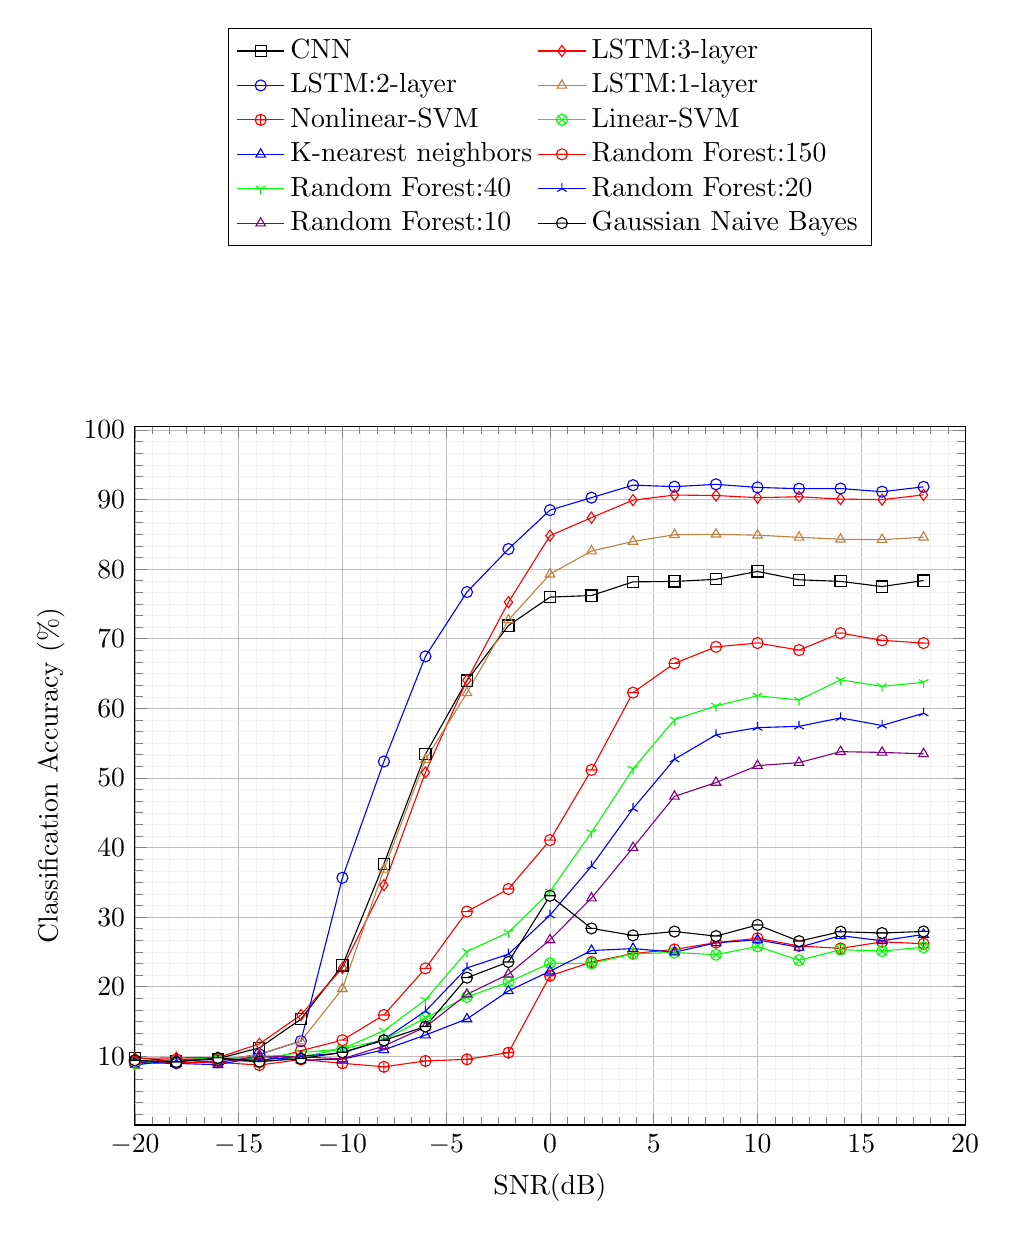
\begin{tikzpicture} \begin{axis}[legend style={at={(0.5,1.57)},anchor=north},
legend columns=2,
 width=\columnwidth,
 grid=both,
 ylabel=Classification Accuracy (\%),
  xlabel=SNR(dB),
 grid style={line width=.1pt, draw=gray!10},
 major grid style={line width=.2pt,draw=gray!50},
 xmin=-20,
 xmax=20,
 %axis lines=middle,
 minor tick num=5,
 legend cell align={left},
 %enlargelimits={abs=0.5},
 %axis line style={latex-latex},
 %ticklabel style={font=\tiny,fill=white},
 %xlabel style={at={(ticklabel* cs:1)},anchor=north west},
 %ylabel style={at={(ticklabel* cs:1)},anchor=south west}
]
%[height=9cm, width=9cm, grid=major,] 
%\addplot {-x^5 - 242}; 
%\addlegendentry{model} 
\addplot[mark=square, color=black] coordinates { 
(-20, 09.807868252516011) (-18, 09.282470481380563) (-16, 09.659913169319827) (-14, 11.205341032118368) (-12, 15.332725615314494) (-10, 23.049582370712635) (-8, 37.6630534631637) (-6, 53.40909090909091) (-4, 63.99260628465804) (-2, 71.89767779390421) (0, 75.98540145985402) (2, 76.20865139949109) (4, 78.1754772393539) (6, 78.23104693140794) (8, 78.53922452660054) (10, 79.67213114754098) (12, 78.47184501176897) (14, 78.2432183059605) (16, 77.50226244343892) (18, 78.36183618361836) };
\addlegendentry{CNN}
\addplot[mark=diamond, color=red] coordinates { 
( -20 , 9.69807868253 )  ( -18 , 9.77293369664 )  ( -16 , 9.80463096961 )  ( -14 , 11.7827499098 )  ( -12 , 15.934366454 )  ( -10 , 22.69415319 )  ( -8 , 34.5948925225 )  ( -6 , 50.7881231672 )  ( -4 , 64.0480591497 )  ( -2 , 75.2539912917 )  ( 0 , 84.8175182482 )  ( 2 , 87.4045801527 )  ( 4 , 89.922907489 )  ( 6 , 90.6498194946 )  ( 8 , 90.5861136159 )  ( 10 , 90.2732240437 )  ( 12 , 90.4037660692 )  ( 14 , 90.071968998 )  ( 16 , 89.9909502262 )  ( 18 , 90.6750675068 )
};
\addlegendentry{LSTM:3-layer}
\addplot[mark=o, color=blue] coordinates {
(-20, 09.387008234217749) (-18, 08.991825613079019) (-16, 09.334298118668596) (-14, 10.285095633345363) (-12, 12.178669097538743) (-10, 35.64954682779456) (-8,  52.36083042439831) (-6,  67.46700879765396) (-4,  76.7097966728281) (-2,  82.89187227866474) (0, 88.48540145985402) (2, 90.27626317702654) (4, 92.0704845814978) (6, 91.85920577617328) (8, 92.19116321009919) (10, 91.74863387978142) (12, 91.56255658156799) (14, 91.58516331426463) (16, 91.13122171945701) (18, 91.82718271827183)
};
\addlegendentry{LSTM:2-layer}
\addplot[mark=triangle, color=brown] coordinates {
(-20, 9.3870082342177488) (-18, 8.9918256130790186) (-16, 9.3342981186685964) (-14,  10.285095633345363) (-12, 12.178669097538743) (-10,19.699166364624865) (-8, 36.863319897398317) (-6, 52.61261261261261) (-4, 62.22222222222222) (-2, 72.69068959209805) (0,  79.27895120174799) (2,  82.60468548238332) (4,  83.97647923557515) (6,  84.94662565587118) (8,  85.01545735588288) (10, 84.88180318856514) (12, 84.57747764190545) (14, 84.29677651719791) (16, 84.23833819241983) (18, 84.59328425210989)
};
\addlegendentry{LSTM:1-layer}
\addplot[mark=oplus, color=red] coordinates {
(  -20 , 9.29551692589 )(  -18 , 9.10081743869 )(  -16 , 9.13531114327 )(  -14 , 8.73330927463 )(  -12 , 9.53509571559 )(  -10 , 8.99235827261 )(  -8 , 8.48796619511 )(  -6 , 9.32917888563 )(  -4 , 9.55637707948 )(  -2 , 10.5224963716 )(  0 , 21.5693430657 )(  2 , 23.5368956743 )(  4 , 24.7613803231 )(  6 , 25.3610108303 )(  8 , 26.3300270514 )(  10 , 26.9581056466 )(  12 , 25.855513308 )(  14 , 25.5028603063 )(  16 , 26.443438914 )(  18 , 26.1746174617 )
};
\addlegendentry{Nonlinear-SVM}
\addplot[mark=otimes, color=green] coordinates {
(  -20 , 9.02104300091 )(  -18 , 9.42779291553 )(  -16 , 9.62373371925 )(  -14 , 9.1122338506 )(  -12 , 9.89972652689 )(  -10 , 11.0716189799 )(  -8 , 12.3461326474 )(  -6 , 15.5241935484 )(  -4 , 18.5212569316 )(  -2 , 20.6640058055 )(  0 , 23.3759124088 )(  2 , 23.3369683751 )(  4 , 24.7246696035 )(  6 , 24.9097472924 )(  8 , 24.5987376014 )(  10 , 25.7923497268 )(  12 , 23.7914177078 )(  14 , 25.3183244141 )(  16 , 25.1221719457 )(  18 , 25.6705670567 )
};
\addlegendentry{Linear-SVM}
\addplot[mark=triangle, color=blue] coordinates {
(  -20 , 9.09423604758 )(  -18 , 8.97366030881 )(  -16 , 8.79160636758 )(  -14 , 9.92421508481 )(  -12 , 9.44393801276 )(  -10 , 9.57881642083 )(  -8 , 10.9314716149 )(  -6 , 13.0498533724 )(  -4 , 15.3604436229 )(  -2 , 19.3940493469 )(  0 , 22.2262773723 )(  2 , 25.1908396947 )(  4 , 25.4772393539 )(  6 , 24.963898917 )(  8 , 26.2939585212 )(  10 , 26.7395264117 )(  12 , 25.6563461887 )(  14 , 27.3297656394 )(  16 , 26.6063348416 )(  18 , 27.5067506751 )
};
\addlegendentry{K-nearest neighbors}
\addplot[mark=halfcircle, color=red] coordinates {
(  -20 , 9.11253430924 )(  -18 , 9.55495004541 )(  -16 , 9.65991316932 )(  -14 , 9.14832190545 )(  -12 , 10.8113035552 )(  -10 , 12.3156211125 )(  -8 , 15.9287157817 )(  -6 , 22.6356304985 )(  -4 , 30.7948243993 )(  -2 , 34.0348330914 )(  0 , 41.0583941606 )(  2 , 51.1450381679 )(  4 , 62.2613803231 )(  6 , 66.4620938628 )(  8 , 68.8367899008 )(  10 , 69.3806921676 )(  12 , 68.3686402318 )(  14 , 70.806421849 )(  16 , 69.7737556561 )(  18 , 69.3789378938 )
};
\addlegendentry{Random Forest:150}
% \addplot[mark=triangle, color=brown] coordinates {
% (  -20 , 9.13083257091 )(  -18 , 10.0454132607 )(  -16 , 9.28002894356 )(  -14 , 9.54529050884 )(  -12 , 10.7019143118 )(  -10 , 11.9246490137 )(  -8 , 15.3040602609 )(  -6 , 20.7661290323 )(  -4 , 28.5767097967 )(  -2 , 31.2409288824 )(  0 , 37.7189781022 )(  2 , 47.8007997092 )(  4 , 59.9853157122 )(  6 , 64.440433213 )(  8 , 67.1956717764 )(  10 , 67.3406193078 )(  12 , 66.6123483614 )(  14 , 68.5366303746 )(  16 , 68.0180995475 )(  18 , 68.0108010801 )
% };
% \addlegendentry{RF:100}
\addplot[mark=Mercedes star flipped, color=green] coordinates {
(  -20 , 8.78316559927 )(  -18 , 9.4459582198 )(  -16 , 9.76845151954 )(  -14 , 9.74377481054 )(  -12 , 10.5013673655 )(  -10 , 11.089390439 )(  -8 , 13.6689325739 )(  -6 , 18.1085043988 )(  -4 , 25.0646950092 )(  -2 , 27.793904209 )(  0 , 33.6678832117 )(  2 , 42.1664849146 )(  4 , 51.3032305433 )(  6 , 58.3754512635 )(  8 , 60.3606853021 )(  10 , 61.8032786885 )(  12 , 61.1986239363 )(  14 , 64.0893153718 )(  16 , 63.149321267 )(  18 , 63.7443744374 )
};
\addlegendentry{Random Forest:40}
\addplot[mark=Mercedes star, color=blue] coordinates {
(  -20 , 8.7648673376 )(  -18 , 9.42779291553 )(  -16 , 9.53328509407 )(  -14 , 9.45507037171 )(  -12 , 10.0091157703 )(  -10 , 10.4673893727 )(  -8 , 12.4196215322 )(  -6 , 16.4772727273 )(  -4 , 22.6987060998 )(  -2 , 24.6734397678 )(  0 , 30.2737226277 )(  2 , 37.3137041076 )(  4 , 45.5947136564 )(  6 , 52.6895306859 )(  8 , 56.1947700631 )(  10 , 57.2313296903 )(  12 , 57.4144486692 )(  14 , 58.6270529618 )(  16 , 57.5384615385 )(  18 , 59.297929793 )
};
\addlegendentry{Random Forest:20}
\addplot[mark=triangle, color=violet] coordinates {
(  -18 , 9.57311534968 )(  -16 , 9.08104196816 )(  -14 , 10.0505232768 )(  -12 , 9.91795806746 )(  -10 , 9.63213079794 )(  -8 , 11.482638251 )(  -6 , 14.2045454545 )(  -4 , 18.9094269871 )(  -2 , 21.7888243832 )(  0 , 26.7153284672 )(  2 , 32.7335514358 )(  4 , 39.9779735683 )(  6 , 47.3465703971 )(  8 , 49.3417493237 )(  10 , 51.766848816 )(  12 , 52.1998913634 )(  14 , 53.7737589961 )(  16 , 53.665158371 )(  18 , 53.4653465347 )
};
\addlegendentry{Random Forest:10}
\addplot[mark=halfcircle, color=black] coordinates {
(  -20 , 9.42360475755 )(  -18 , 9.17347865577 )(  -16 , 9.76845151954 )(  -14 , 9.23854204258 )(  -12 , 9.66271649954 )(  -10 , 10.5740181269 )(  -8 , 12.2910159838 )(  -6 , 14.2778592375 )(  -4 , 21.2939001848 )(  -2 , 23.5486211901 )(  0 , 33.0656934307 )(  2 , 28.3715012723 )(  4 , 27.3678414097 )(  6 , 27.9241877256 )(  8 , 27.2678088368 )(  10 , 28.8706739526 )(  12 , 26.5435451747 )(  14 , 27.9018269053 )(  16 , 27.7104072398 )(  18 , 27.9387938794 )
};
\addlegendentry{Gaussian Naive Bayes}
\addplot[mark=triangle, color=brown] coordinates {
};
\addlegendentry{MNB}
\addplot[mark=triangle, color=brown] coordinates {

};
\addlegendentry{SVC}
\end{axis}
\end{tikzpicture}
\caption{Classification accuracy comparison of hyper-parameter optimized 2-layer amplitude-phase \ac{lstm} model with others on RadioML dataset.}
%\label{fig_rml_comp_acc}
\label{fig_lstm_rml_acc}
\end{figure}

\begin{figure}[htb]
\centering
-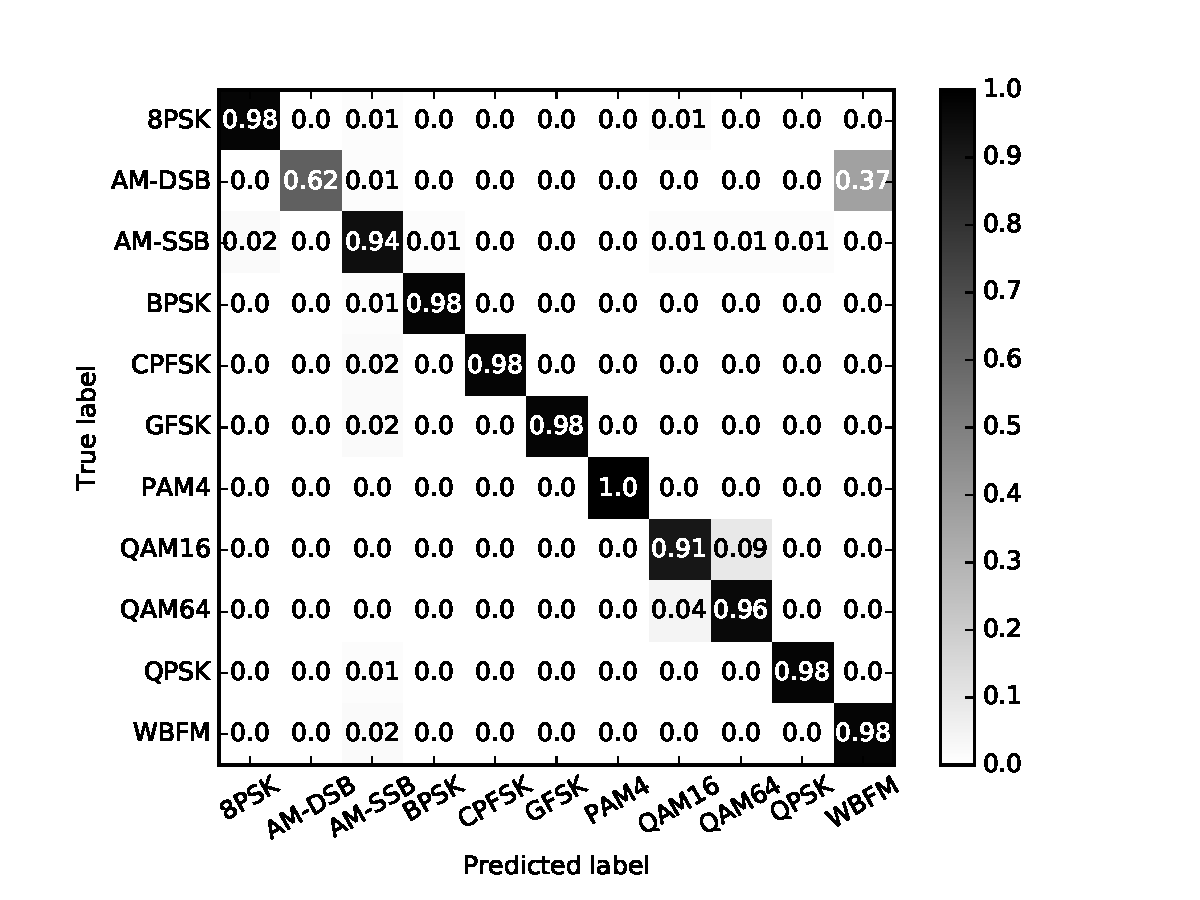
\includegraphics[width=1.1\columnwidth]{figures/confmat_18.pdf}
\caption{Confusion matrix for 2-layer amplitude-phase LSTM model on RadioML dataset at 18dB SNR} 
\label{fig_confmat_18}
\end{figure}

\begin{figure}[htb]
\centering
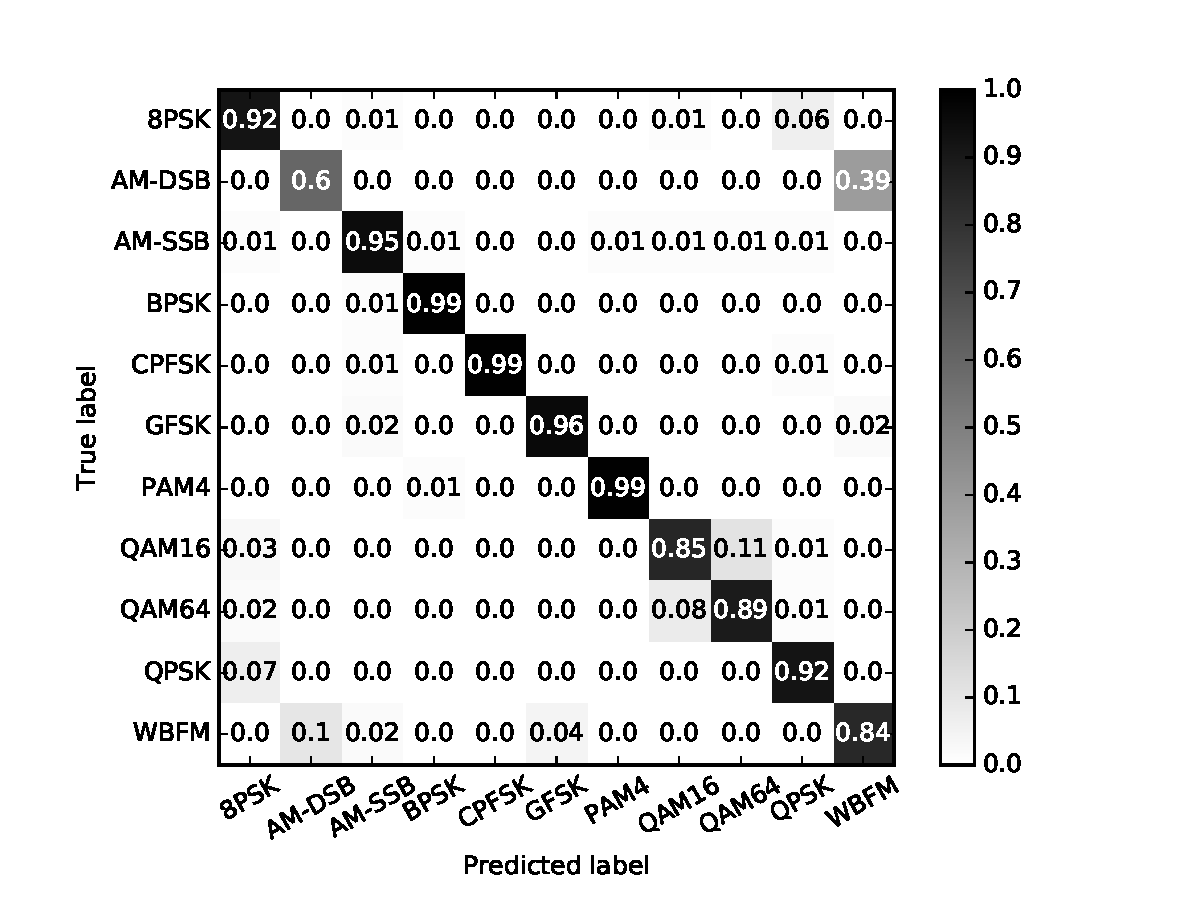
\includegraphics[width=1.1\columnwidth]{figures/confmat_0.pdf}
\caption{Confusion matrix for 2-layer amplitude-phase LSTM model on RadioML dataset at 0dB SNR} 
\label{fig_confmat_0}
\end{figure}

\begin{figure}[htb]
\centering
\squeezeup
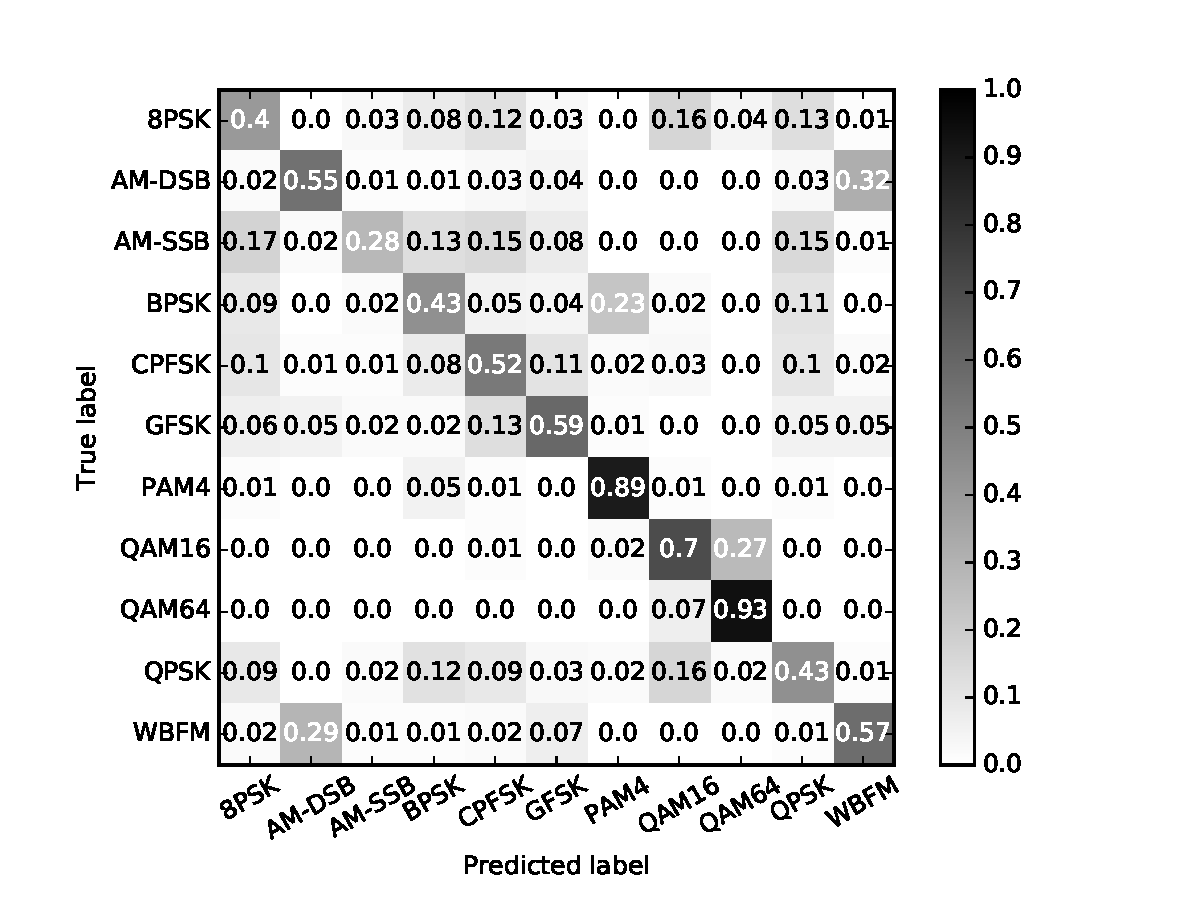
\includegraphics[width=1.1\columnwidth]{figures/confmat_-8.pdf}
\caption{Confusion matrix for 2-layer amplitude-phase LSTM model on RadioML dataset at -8dB SNR} 
\label{fig_confmat_-8}
\end{figure}

\begin{figure}[htb]
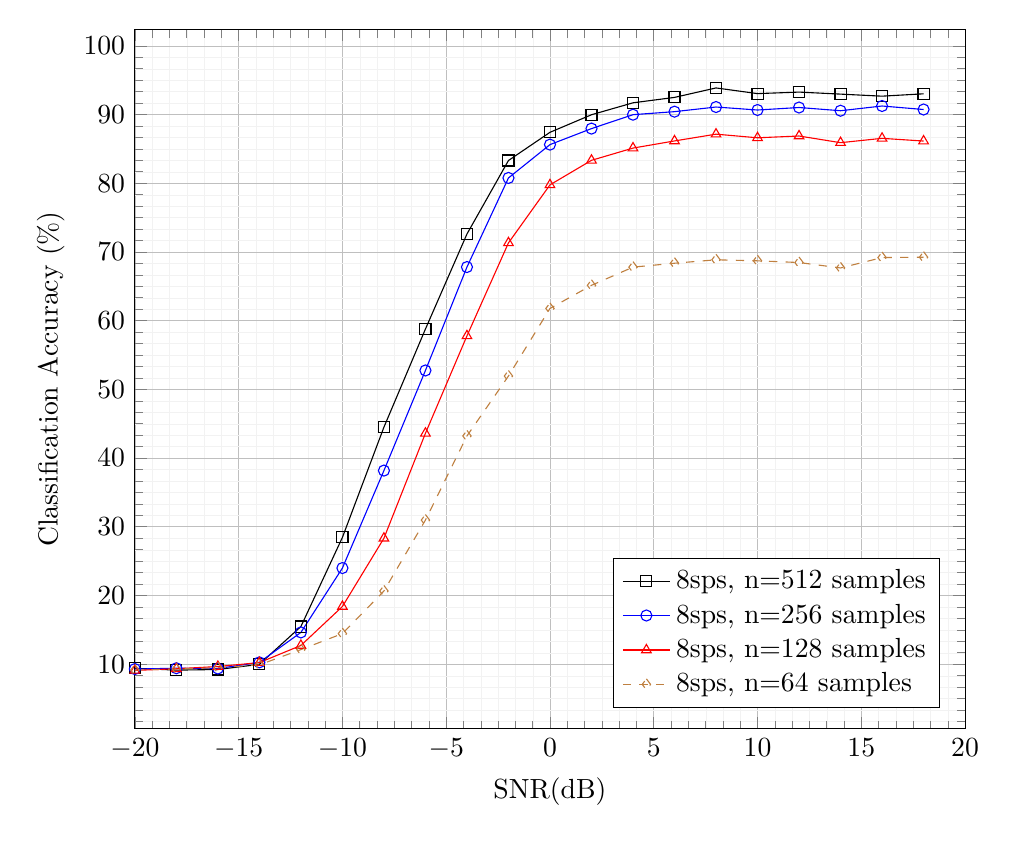
\begin{tikzpicture} \begin{axis}[legend pos=south east,
 width=\columnwidth,
 grid=both,
 ylabel=Classification Accuracy (\%),
  xlabel=SNR(dB),
 grid style={line width=.1pt, draw=gray!10},
 major grid style={line width=.2pt,draw=gray!50},
 minor tick num=5,
 xmin=-20,
 xmax=20,
 legend cell align={left},
]
\addplot[mark=square, color=black] coordinates {
(-20, 09.405306495882891) (-18, 09.137148047229791) (-16, 09.225759768451519) (-14, 09.978347167087694) (-12, 15.478577939835916) (-10, 28.45210591789586) (-8,  44.497519750137793) (-6,  58.77932551319648) (-4,  72.60628465804067) (-2,  83.30914368650217) (0,   87.40875912408759) (2,   89.96728462377317) (4,   91.70337738619677) (6,   92.49097472924188) (8,   93.86834986474302) (10,  93.04189435336976) (12,  93.26453014665942) (14,  92.96918250599742) (16,  92.66968325791856) (18,  93.01530153015302)
};
\addlegendentry{8sps, n=512 samples}
\addplot[mark=o, color=blue] coordinates {
(-20, 09.29551692589204) (-18, 09.409627611262489) (-16, 09.370477568740955) (-14, 10.267051605918441) (-12, 14.62169553327256) (-10, 23.991469699662343) (-8,  38.17747565680691) (-6,  52.74926686217009) (-4,  67.8003696857671) (-2,  80.76923076923077) (0,   85.62043795620438) (2,   87.94983642311887) (4,   89.97797356828194) (6,   90.41516245487364) (8,   91.09107303877367) (10,  90.65573770491804) (12,  91.01937352887923) (14,  90.55176231777081) (16,  91.23981900452489) (18,  90.72907290729073)
};
\addlegendentry{8sps, n=256 samples}
\addplot[mark=triangle, color=red] coordinates {
(-20, 09.09423604757548) (-18, 09.336966394187103) (-16, 09.659913169319827) (-14, 10.230963551064598) (-12, 12.725615314494074) (-10, 18.393460103074463) (-8,  28.32996509277972) (-6,  43.603372434017595) (-4,  57.7818853974122) (-2,  71.31712626995645) (0,   79.76277372262773) (2,   83.33333333333334) (4,   85.11380323054332) (6,   86.15523465703971) (8,   87.14156898106402) (10,  86.61202185792349) (12,  86.8730762266884) (14,  85.90145783354862) (16,  86.53393665158371) (18,  86.13861386138614)
};
\addlegendentry{8sps, n=128 samples}
\addplot[dashed, mark=diamond, color=brown] coordinates {
(-20, 09.149130832570906) (-18, 09.30063578564941) (-16, 09.479015918958032) (-14, 09.906171057380007) (-12, 12.123974475843209) (-10, 14.448196196907767) (-8,  20.65037663053463) (-6,  30.97507331378299) (-4,  43.21626617375231) (-2,  51.94121915820029) (0,   61.77007299270073) (2,   65.13994910941476) (4,   67.7863436123348) (6,   68.35740072202167) (8,   68.85482416591524) (10,  68.70673952641165) (12,  68.45917074053957) (14,  67.66931168112198) (16,  69.1764705882353) (18,  69.23492349234923)
};
\addlegendentry{8sps, n=64 samples}
\end{axis}
\end{tikzpicture}
\caption{Classification accuracy of amplitude-phase \ac{lstm} model on modified RadioML dataset for 8 samples/symbol. The model is trained only on input sample lengths (n) from 128 to 512. The model gives close to 70\% accuracy on 64 input samples (dashed line) which it is not trained for. }
\label{fig_lstm_modrml_acc_8sps}
\end{figure}


\begin{figure}[htb]
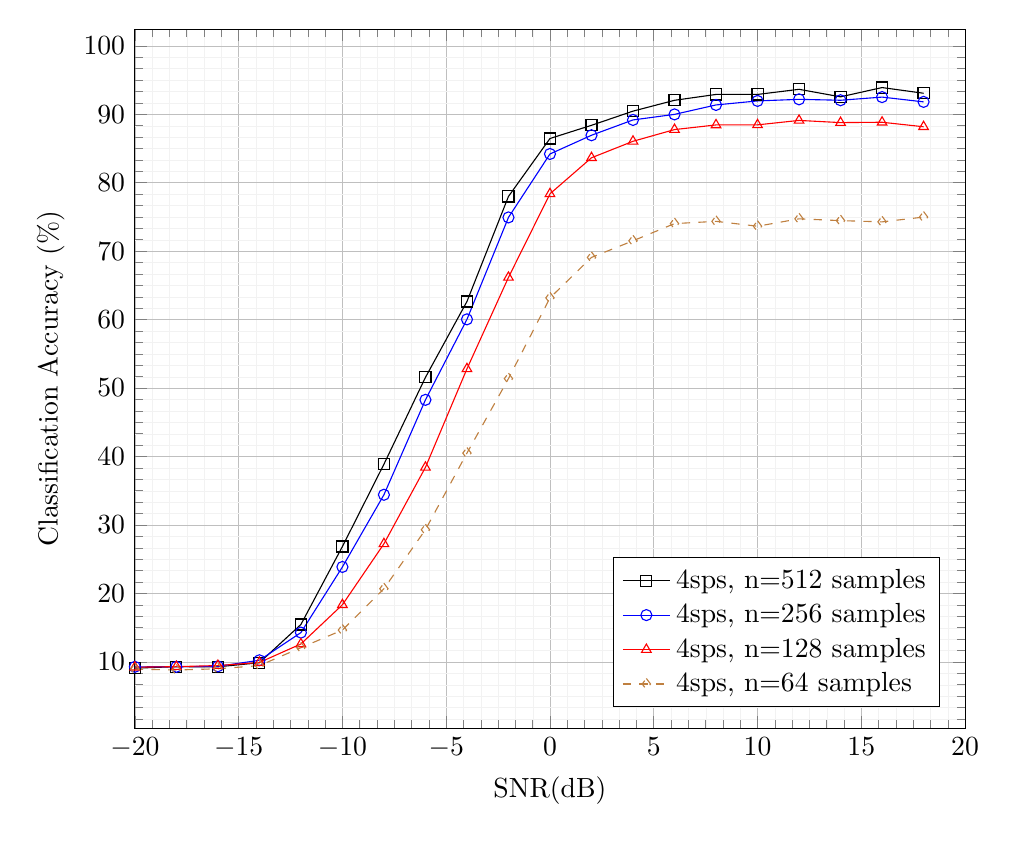
\begin{tikzpicture} \begin{axis}[legend pos=south east,
 width=\columnwidth,
 grid=both,
 ylabel=Classification Accuracy (\%),
  xlabel=SNR(dB),
 grid style={line width=.1pt, draw=gray!10},
 major grid style={line width=.2pt,draw=gray!50},
 minor tick num=5,
 xmin=-20,
 xmax=20,
 legend cell align={left},
]
\addplot[mark=square, color=black] coordinates {
(-20, 09.075937785910339) (-18, 09.30063578564941) (-16, 09.280028943560058) (-14, 09.870083002526164) (-12, 15.460346399270739) (-10, 26.852674604585036) (-8,  38.875620062465555) (-6,  51.55791788856305) (-4,  62.64325323475046) (-2,  77.99346879535559) (0,   86.45985401459854) (2,   88.38604143947656) (4,   90.45521292217328) (6,   92.03971119133574) (8,   92.89449954914337) (10,  92.89617486338798) (12,  93.64475828354155) (14,  92.54474995386602) (16,  93.90045248868778) (18,  93.06930693069307)
};
\addlegendentry{4sps, n=512 samples}
\addplot[mark=o, color=blue] coordinates {
(-20, 09.277218664226898) (-18, 09.282470481380563) (-16, 09.352387843704775) (-14, 10.230963551064598) (-12, 14.275296262534184) (-10, 23.867069486404835) (-8,  34.41117031049054) (-6,  48.277126099706746) (-4,  60.03696857670979) (-2,  74.92743105950653) (0,   84.1970802919708) (2,   86.93202471828426) (4,   89.17033773861968) (6,   89.98194945848376) (8,   91.36158701532913) (10,  91.94899817850638) (12,  92.17816404128191) (14,  92.04650304484222) (16,  92.50678733031674) (18,  91.8091809180918)
};
\addlegendentry{4sps, n=256 samples}
\addplot[mark=triangle, color=red] coordinates {
(-20, 09.222323879231473) (-18, 09.30063578564941) (-16, 09.460926193921852) (-14, 09.906171057380007) (-12, 12.61622607110301) (-10, 18.340145725964102) (-8,  27.246004041888666) (-6,  38.41642228739003) (-4,  52.80961182994455) (-2,  66.16473149492017) (0,   78.37591240875912) (2,   83.6423118865867) (4,   86.04992657856094) (6,   87.76173285198556) (8,   88.4400360685302) (10,  88.45173041894353) (12,  89.10012674271229) (14,  88.78021775235283) (16,  88.83257918552037) (18,  88.17281728172818)
};
\addlegendentry{4sps, n=128 samples}
\addplot[dashed, mark=diamond, color=brown] coordinates {
(-20, 08.947849954254346) (-18, 08.810172570390554) (-16, 08.990593342981186) (-14, 09.455070371706965) (-12, 12.069279854147676) (-10, 14.643682246312423) (-8,  20.687121072937717) (-6,  29.30718475073314) (-4,  40.499075785582256) (-2,  51.37880986937591) (0,   63.17518248175182) (2,   69.08396946564885) (4,   71.51248164464024) (6,   74.02527075812274) (8,   74.35527502254283) (10,  73.64298724954462) (12,  74.72388194821655) (14,  74.46023251522421) (16,  74.28054298642534) (18,  74.97749774977498)
};
\addlegendentry{4sps, n=64 samples}
\end{axis}
\end{tikzpicture}
\caption{Classification accuracy  of amplitude-phase \ac{lstm} model on modified RadioML dataset for 4 samples/symbol. The model is trained only on input sample lengths (n) from 128 to 512. The model gives close to 75\% accuracy on 64 input samples (dashed line) which it is not trained for.}
\label{fig_lstm_modrml_acc_4sps}
\end{figure}

\begin{figure}[htb]
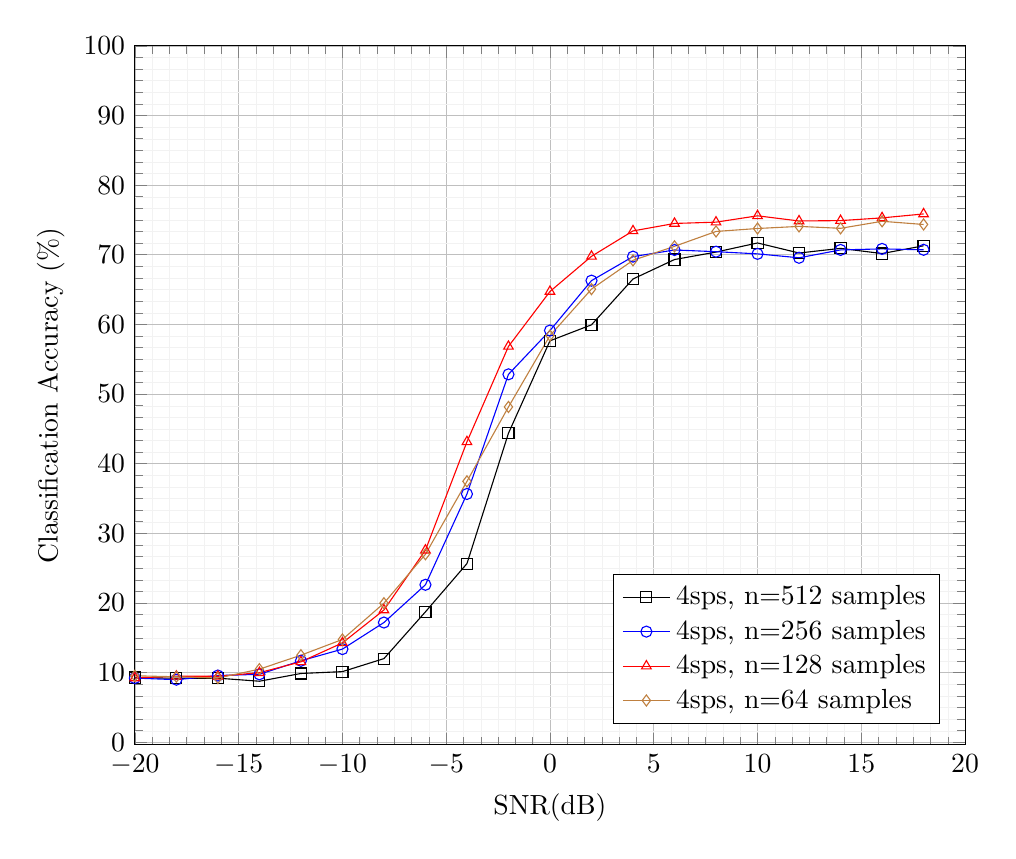
\begin{tikzpicture} \begin{axis}[legend pos=south east,
 width=\columnwidth,
 grid=both,
 ylabel=Classification Accuracy (\%),
  xlabel=SNR(dB),
 grid style={line width=.1pt, draw=gray!10},
 major grid style={line width=.2pt,draw=gray!50},
 minor tick num=5,
 xmin=-20,
 xmax=20,
 ymax=100,
 legend cell align={left},
]

\addplot[mark=square, color=black] coordinates {
(  -20 , 9.29551692589 )(  -18 , 9.19164396004 )(  -16 , 9.20767004342 )(  -14 , 8.76939732948 )(  -12 , 9.88149498633 )(  -10 , 10.14750311 )(  -8 , 12.0154326658 )(  -6 , 18.7316715543 )(  -4 , 25.6561922366 )(  -2 , 44.3759071118 )(  0 , 57.6459854015 )(  2 , 59.9418393312 )(  4 , 66.5198237885 )(  6 , 69.3140794224 )(  8 , 70.3877366997 )(  10 , 71.693989071 )(  12 , 70.2516748144 )(  14 , 70.9171433844 )(  16 , 70.1719457014 )(  18 , 71.2871287129 )
};
\addlegendentry{4sps, n=512 samples}
\addplot[mark=o, color=blue] coordinates {
(  -20 , 9.22232387923 )(  -18 , 8.99182561308 )(  -16 , 9.58755426918 )(  -14 , 9.76181883796 )(  -12 , 11.7046490428 )(  -10 , 13.3819086547 )(  -8 , 17.1963990446 )(  -6 , 22.6173020528 )(  -4 , 35.6561922366 )(  -2 , 52.8301886792 )(  0 , 59.1240875912 )(  2 , 66.2849872774 )(  4 , 69.7320117474 )(  6 , 70.6859205776 )(  8 , 70.441839495 )(  10 , 70.1275045537 )(  12 , 69.5636429477 )(  14 , 70.6957003137 )(  16 , 70.8416289593 )(  18 , 70.7110711071 )
};
\addlegendentry{4sps, n=256 samples}
\addplot[mark=triangle, color=red] coordinates {
(  -20 , 9.2406221409 )(  -18 , 9.48228882834 )(  -16 , 9.47901591896 )(  -14 , 9.99639119451 )(  -12 , 11.5587967183 )(  -10 , 14.2704816065 )(  -8 , 18.9968767224 )(  -6 , 27.5843108504 )(  -4 , 43.1423290203 )(  -2 , 56.8396226415 )(  0 , 64.7262773723 )(  2 , 69.7746274082 )(  4 , 73.4214390602 )(  6 , 74.4945848375 )(  8 , 74.6798917944 )(  10 , 75.5919854281 )(  12 , 74.8506246605 )(  14 , 74.9031186566 )(  16 , 75.2941176471 )(  18 , 75.8595859586 )

};
\addlegendentry{4sps, n=128 samples}
\addplot[mark=diamond, color=brown] coordinates {
(  -20 , 9.5516925892 )(  -18 , 9.40962761126 )(  -16 , 9.22575976845 )(  -14 , 10.5016239625 )(  -12 , 12.5068368277 )(  -10 , 14.7680824596 )(  -8 , 19.9706044461 )(  -6 , 26.9978005865 )(  -4 , 37.4676524954 )(  -2 , 48.1494920174 )(  0 , 58.3941605839 )(  2 , 65.0672482734 )(  4 , 69.1997063142 )(  6 , 71.2093862816 )(  8 , 73.3453561767 )(  10 , 73.7704918033 )(  12 , 74.072062285 )(  14 , 73.7959033032 )(  16 , 74.8054298643 )(  18 , 74.3474347435 )
};
\addlegendentry{4sps, n=64 samples}



% \addplot[mark=square, color=black] coordinates {
% (  -20 , 9.5516925892 )(  -18 , 9.40962761126 )(  -16 , 9.22575976845 )(  -14 , 10.5016239625 )(  -12 , 12.5068368277 )(  -10 , 14.7680824596 )(  -8 , 19.9706044461 )(  -6 , 26.9978005865 )(  -4 , 37.4676524954 )(  -2 , 48.1494920174 )(  0 , 58.3941605839 )(  2 , 65.0672482734 )(  4 , 69.1997063142 )(  6 , 71.2093862816 )(  8 , 73.3453561767 )(  10 , 73.7704918033 )(  12 , 74.072062285 )(  14 , 73.7959033032 )(  16 , 74.8054298643 )(  18 , 74.3474347435 )
% };
% \addlegendentry{4sps, n=64 samples}
% \addplot[mark=o, color=blue] coordinates {
% (  -20 , 9.2406221409 )(  -18 , 9.48228882834 )(  -16 , 9.47901591896 )(  -14 , 9.99639119451 )(  -12 , 11.5587967183 )(  -10 , 14.2704816065 )(  -8 , 18.9968767224 )(  -6 , 27.5843108504 )(  -4 , 43.1423290203 )(  -2 , 56.8396226415 )(  0 , 64.7262773723 )(  2 , 69.7746274082 )(  4 , 73.4214390602 )(  6 , 74.4945848375 )(  8 , 74.6798917944 )(  10 , 75.5919854281 )(  12 , 74.8506246605 )(  14 , 74.9031186566 )(  16 , 75.2941176471 )(  18 , 75.8595859586 )

% };
% \addlegendentry{4sps, n=128 samples}
% \addplot[mark=triangle, color=red] coordinates {
% (  -20 , 9.22232387923 )(  -18 , 8.99182561308 )(  -16 , 9.58755426918 )(  -14 , 9.76181883796 )(  -12 , 11.7046490428 )(  -10 , 13.3819086547 )(  -8 , 17.1963990446 )(  -6 , 22.6173020528 )(  -4 , 35.6561922366 )(  -2 , 52.8301886792 )(  0 , 59.1240875912 )(  2 , 66.2849872774 )(  4 , 69.7320117474 )(  6 , 70.6859205776 )(  8 , 70.441839495 )(  10 , 70.1275045537 )(  12 , 69.5636429477 )(  14 , 70.6957003137 )(  16 , 70.8416289593 )(  18 , 70.7110711071 )
% };
% \addlegendentry{4sps, n=256 samples}
% \addplot[mark=diamond, color=brown] coordinates {
% (  -20 , 9.29551692589 )(  -18 , 9.19164396004 )(  -16 , 9.20767004342 )(  -14 , 8.76939732948 )(  -12 , 9.88149498633 )(  -10 , 10.14750311 )(  -8 , 12.0154326658 )(  -6 , 18.7316715543 )(  -4 , 25.6561922366 )(  -2 , 44.3759071118 )(  0 , 57.6459854015 )(  2 , 59.9418393312 )(  4 , 66.5198237885 )(  6 , 69.3140794224 )(  8 , 70.3877366997 )(  10 , 71.693989071 )(  12 , 70.2516748144 )(  14 , 70.9171433844 )(  16 , 70.1719457014 )(  18 , 71.2871287129 )
% };
% \addlegendentry{4sps, n=512 samples}
\end{axis}
\end{tikzpicture}
\caption{Classification accuracy  of amplitude-phase \ac{lstm} model for non-trained data lengths on modified RadioML dataset with 4 samples/symbol.}
\label{fig_lstm_modrml_generalization}
\end{figure}

\begin{figure*}[!t]
\centering
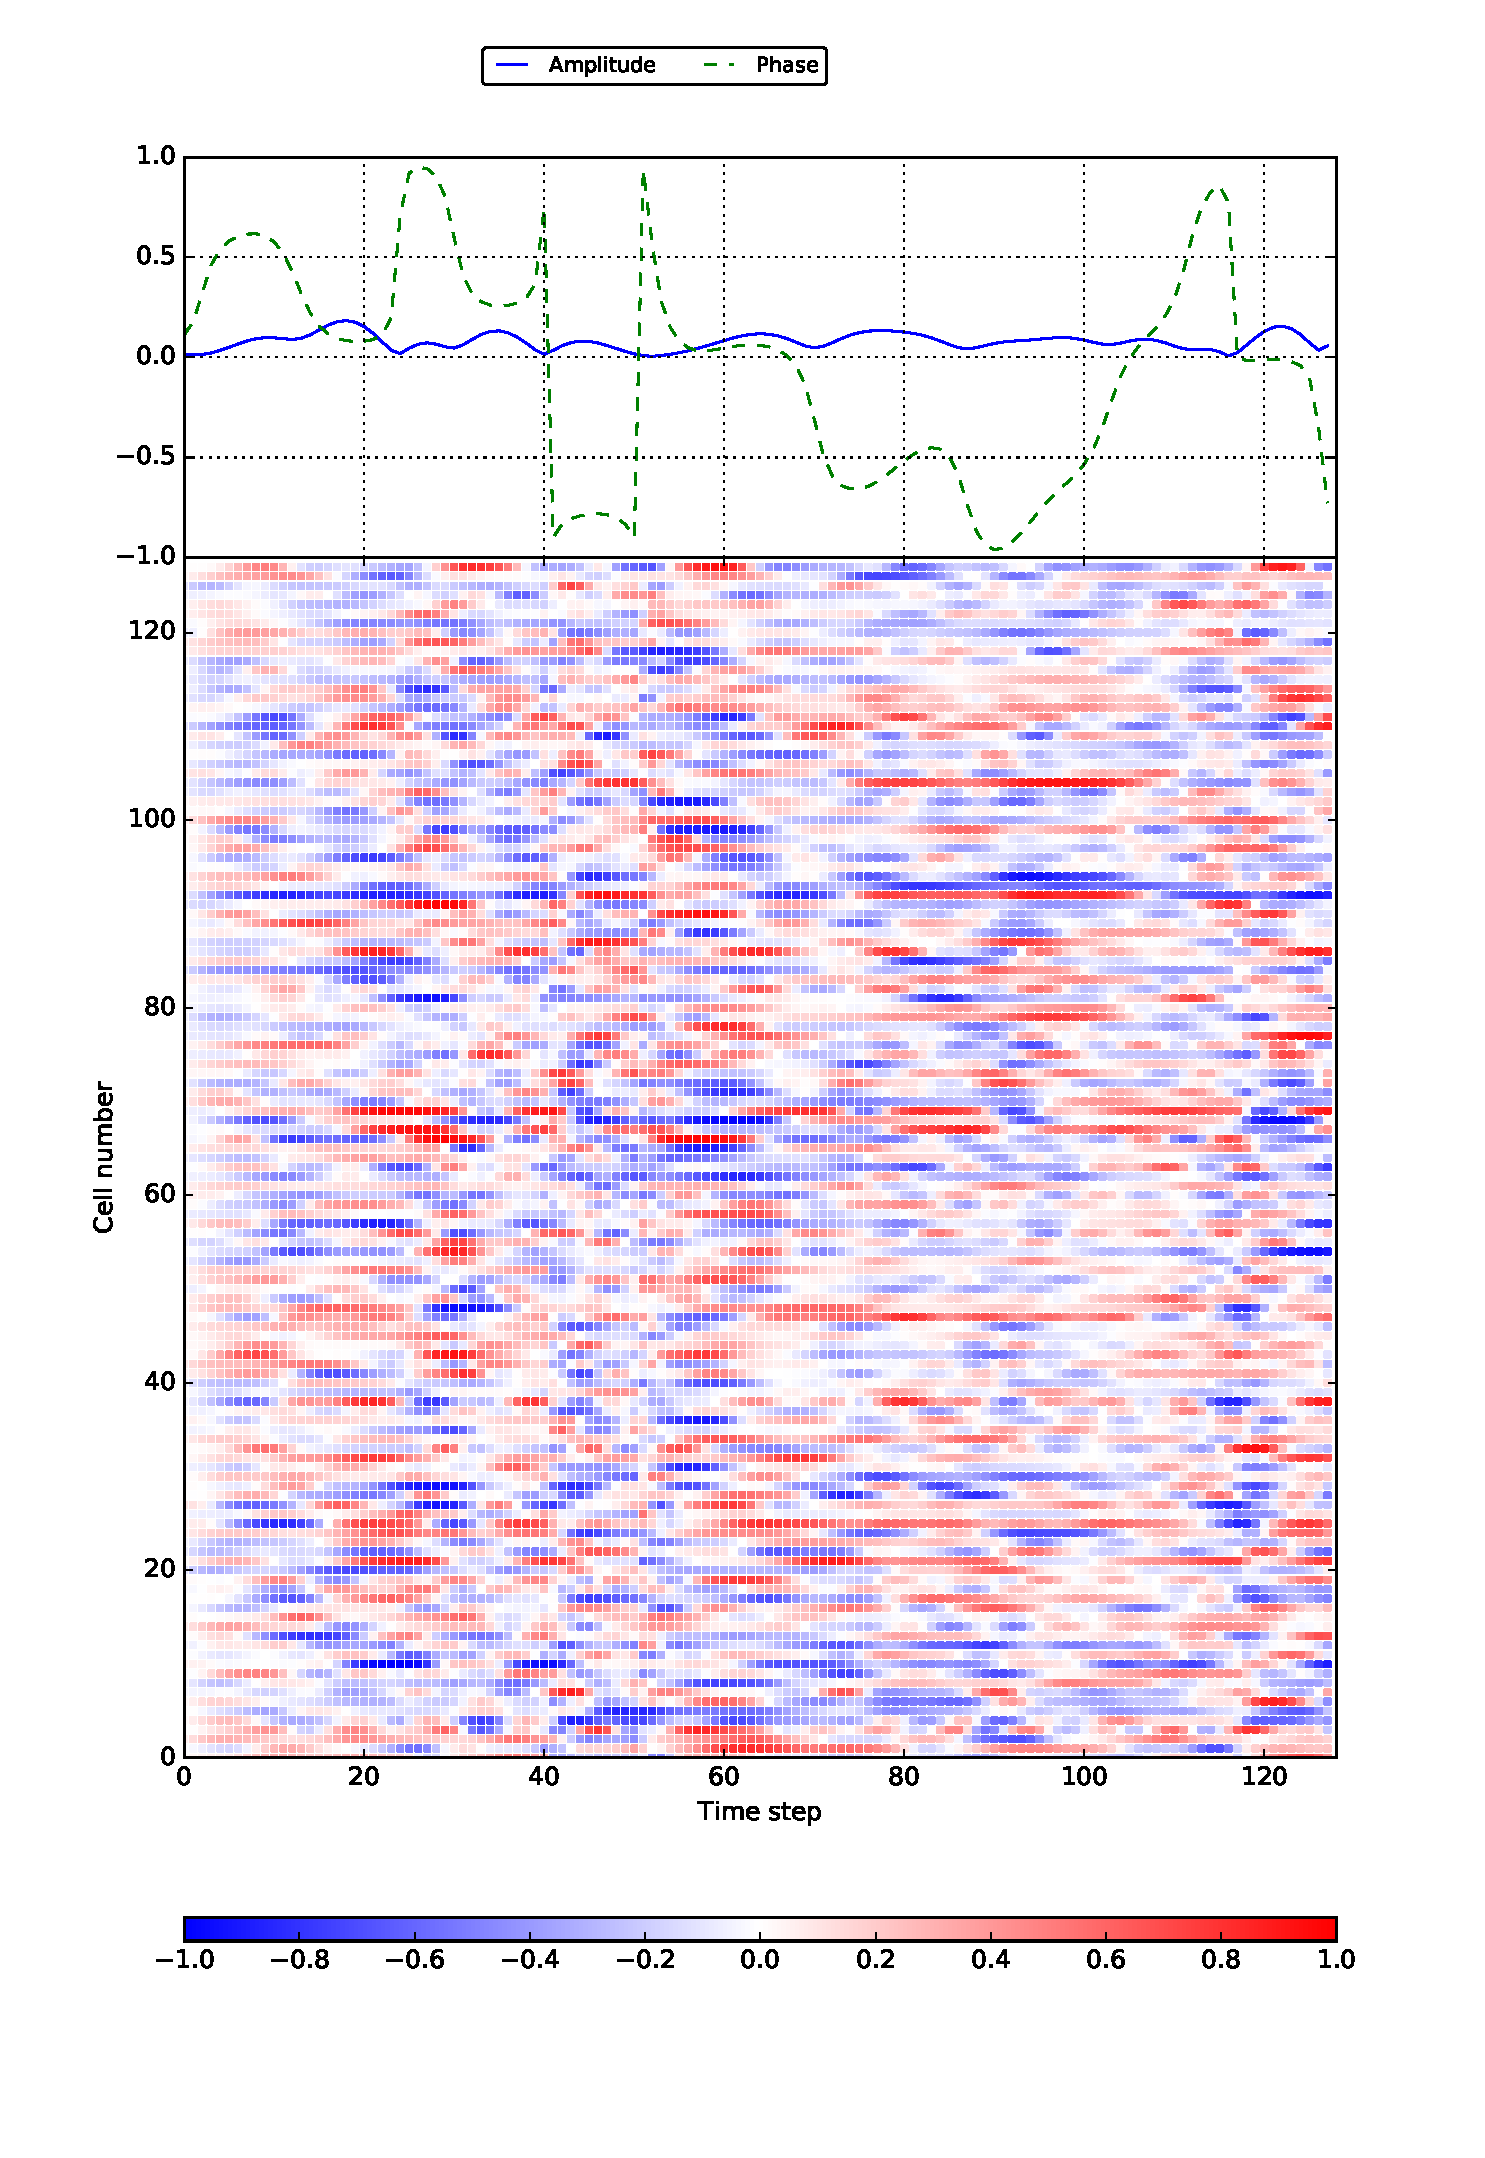
\includegraphics[width=1\columnwidth]{figures/layer_1_new1.pdf}
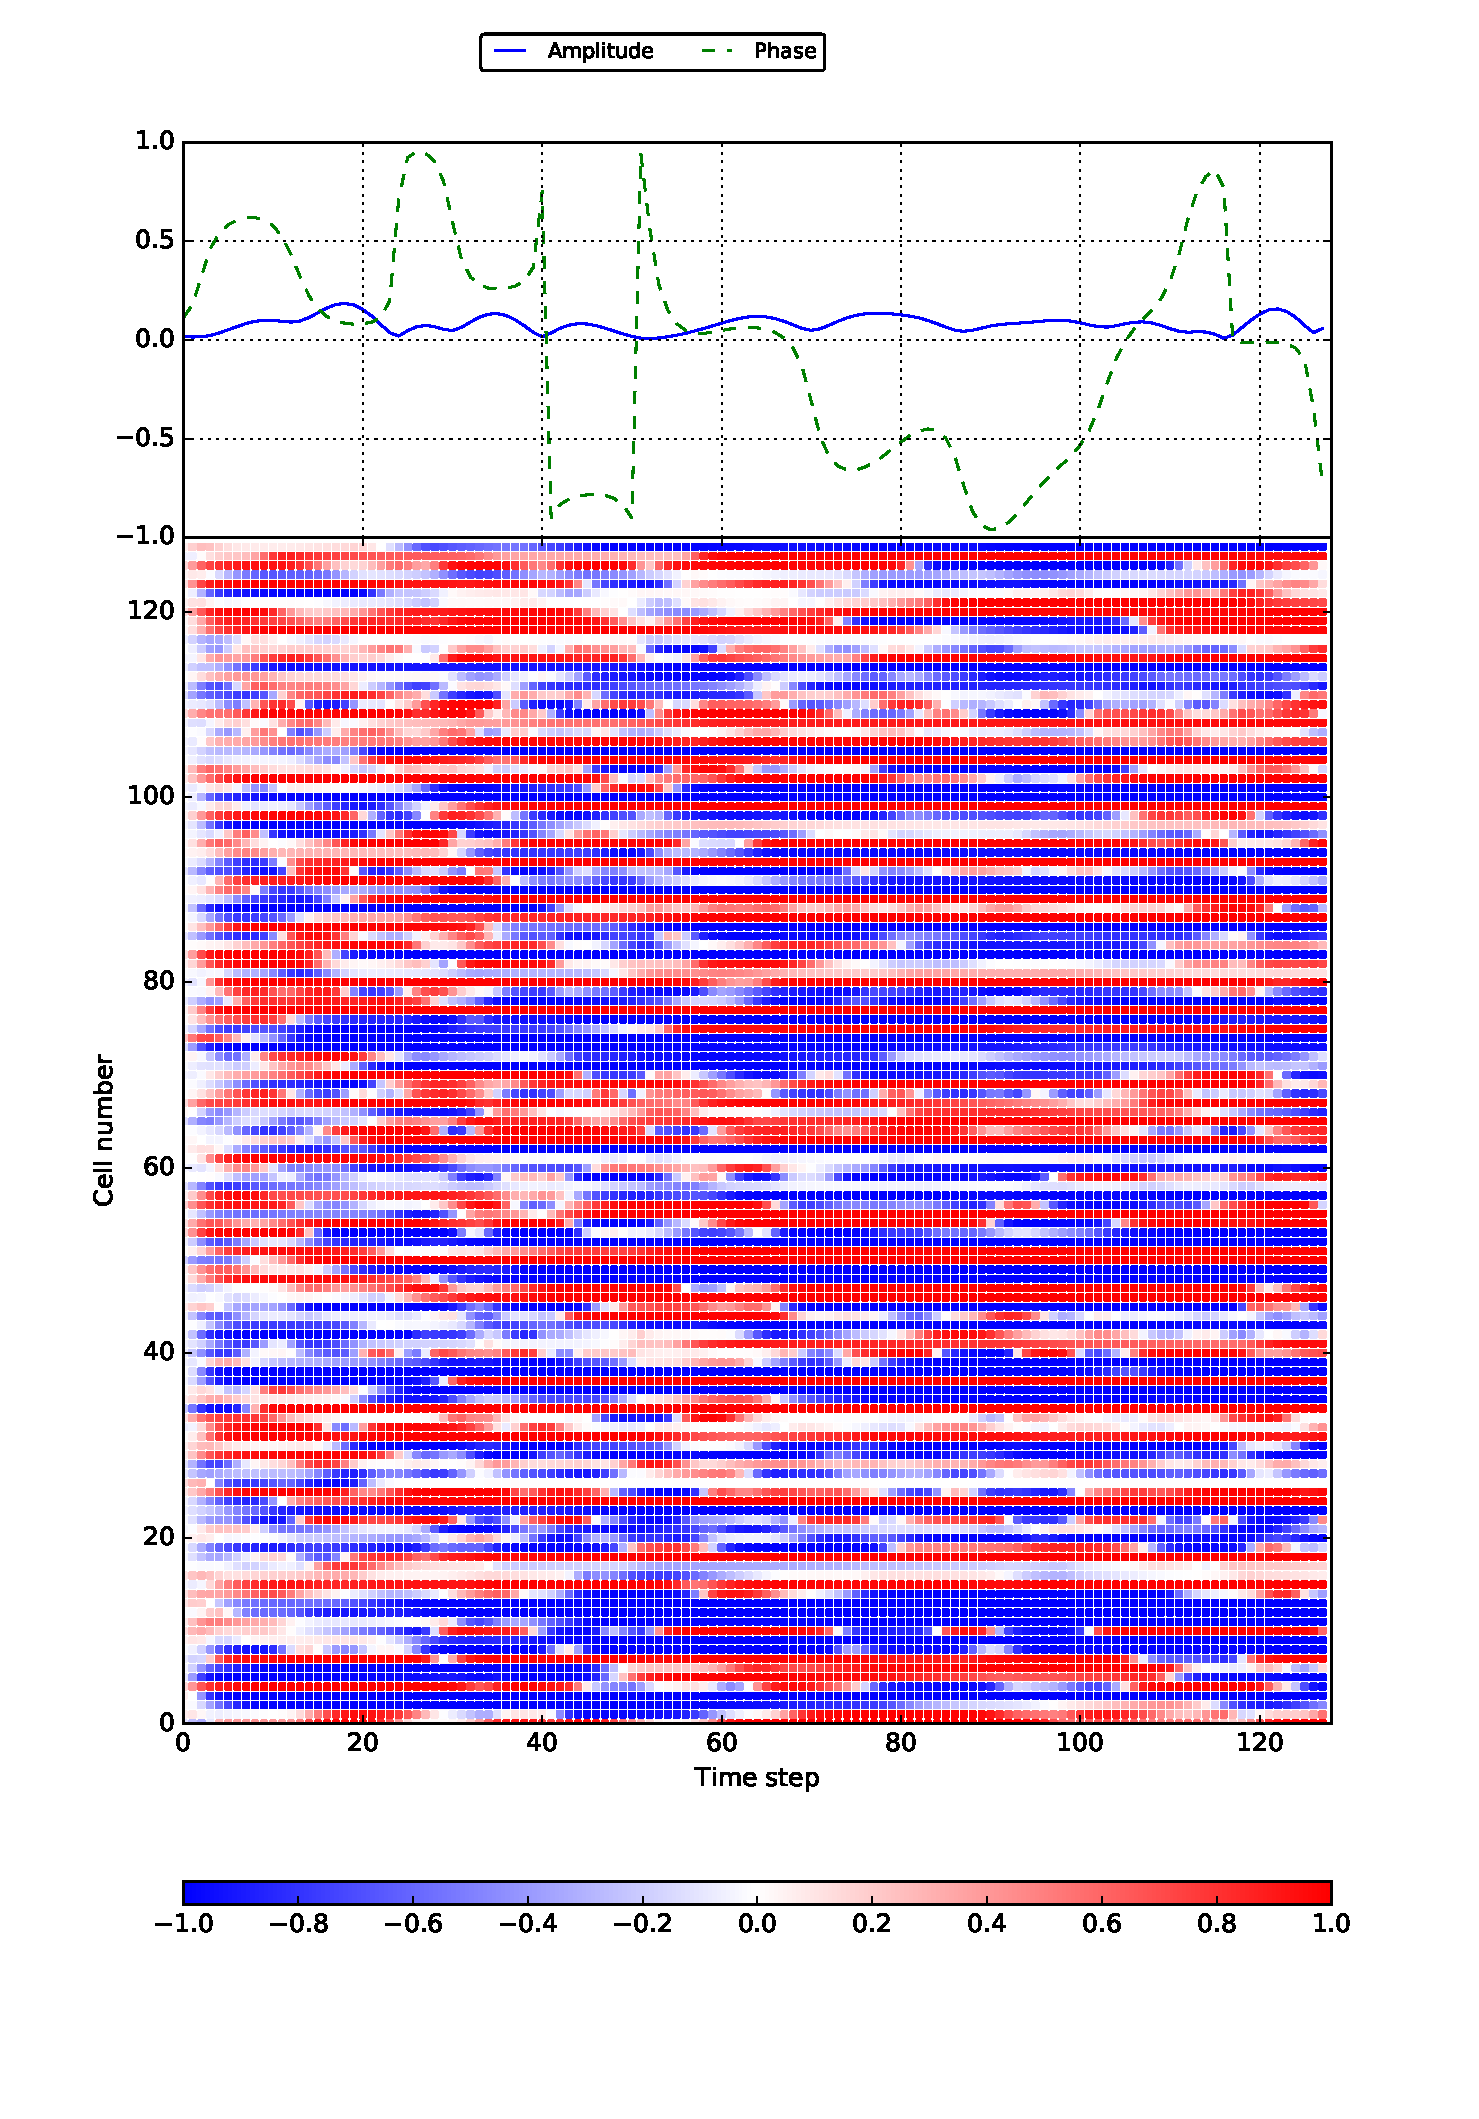
\includegraphics[width=1\columnwidth]{figures/layer_2_new1.pdf}
\caption{Layer-1 (left) and layer-2 (right) LSTM temporal activations for a QAM64 input vector. On the top the amplitude and phase of the input signal (y-axis) is plotted at each time step (x-axis). Below the amplitude and phase of the signal, temporal activations for all cells in the \ac{lstm} model for each time step are shown. Blue denotes \textit{tanh(c)} activations of value -1 and red denotes a value of +1.} 
\label{fig_activations}
\end{figure*}

\begin{figure*}[!t]
\centering
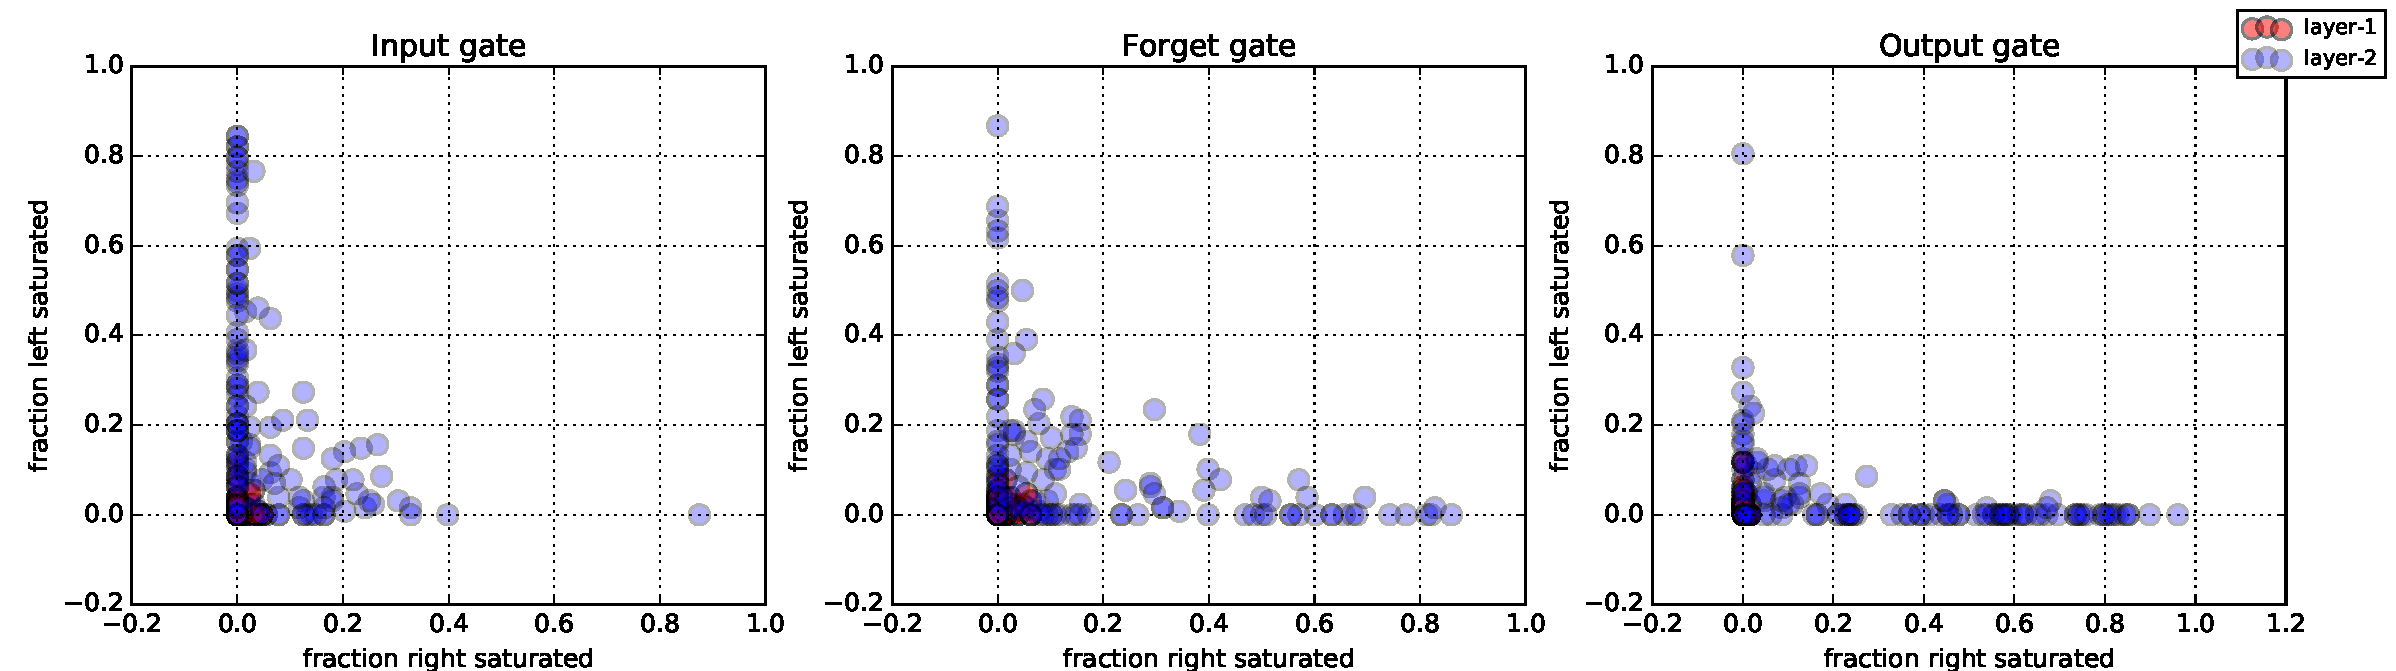
\includegraphics[width=2\columnwidth]{figures/gate_sat.pdf}
\caption{Gate saturation plots for LSTM for the same a QAM64 input vector. A circle represents a gate in a particular LSTM cell.} 
\label{fig_gatesat}
\end{figure*}



\subsection{Classification accuracy on RadioML dataset}
%\vincent{At the end of Section V.A, you mention how your normalize the amplitude and phase for the input to the model. This information should already be provided in Section IV as it seems an important design decision.}
The two layer amplitude-phase \ac{lstm} model, shown in Figure~\ref{fig_iq_lstm_model}, is trained on SNR ranges from -10dB to 20dB. Training vectors with SNR ranges below -10dB were not used as the model was converging slowly when those vectors were used. Alternate models with varying \ac{lstm} layer depths are also trained to understand the performance improvements provided by the different layer depths. The classification accuracy of all the four models are presented in Figure~\ref{fig_lstm_rml_acc}. The two layer \ac{lstm} model gave an average accuracy of 90\% in \ac{snr} ranges from 0dB to 20dB. It can be noticed that the single layer \ac{lstm} also reaches a high accuracy at high \ac{snr}s, 6\% less than the two layer model. It was also noticed that the classification accuracy saturates for layer depths of two. Hence, layer depth of two is selected for the final model and its parameters are fine tuned (dropout = 0.8 and learning rate = 0.001) to achieve the best test performance as shown in Figure~\ref{fig_lstm_rml_acc}. Rigorous fine tuning was not performed on layer depths other than two accounting for a slightly lower accuracy levels, for instance the accuracy level for layer depth 3 is slightly lower than layer depth two.  The performance of the baseline \ac{cnn} model was shown to be much better on the low \ac{snr} regions in \cite{baseline}. We were not able to reproduce the reported results on the low \ac{snr} regions after various attempts, which may be because of the difference in hyper-parameter tuning. Though, the high \ac{snr} results of the baseline model matches with that of the reported ones in the paper. Detailed discussions on the effect of layer depth and number of \ac{lstm} cells are presented in Section~\ref{sec_hyperparams}.

Classification performance of other standard machine learning models such as \ac{svm}, random forest, k-nearest neighbors and Gaussian Naive Bayes are also summarized in Figure~\ref{fig_lstm_rml_acc}. All models are fed with the same amplitude-phase training and test data for this comparison. Random forest with 150 decision trees is able to provide close to 70\% of accuracy at very high \ac{snr} conditions while others could reach only around 26\%. It could be clearly noticed that the deep learning models perform superior to the other standard techniques when fed with the raw sensed data. The deep learning models can classify signals very efficiently with a very low number of symbols, usually with hundreds of samples (tens of modulated symbols) when compared to the classical cyclostationary based expert feature models which requires samples in thousands range (hundreds of modulated symbols) for averaging. Similarly extracting expert cyclostationary features using tens of symbols is very suboptimal, which substantiate the use of deep learning models.

To understand the results better confusion matrices for the two layer \ac{lstm} model for various \ac{snr}s are also included. It can be seen in Figure~\ref{fig_confmat_18} that at a high \ac{snr} of 18dB the diagonal is much more sharp even though there are difficulties in separating AM-DSB and WBFM signals. This is mainly due to the silence periods of audio as the modulated signals are generated from real audio streams.  Similarly in Figure~\ref{fig_confmat_0}, at 0dB \ac{snr} it is noticed that there is some level of confusion regarding QAM16 and QAM64 as the former is a subset of the the latter. The confusion increases further at low \ac{snr}s as shown in Figure~\ref{fig_confmat_-8}. From these basic analysis it is clear that deep complex structures as mentioned in \cite{baseline} are not required to achieved good \ac{soa} classification accuracy at high \ac{snr}s. However, use of convolutional layers might turn useful at low \ac{snr}s as reported in \cite{baseline}. In our experiments we also noticed that simply providing \ac{iq} samples to the \ac{lstm} model yielded poor results while normalized amplitude and phase interpretation provided good results. The models even failed to reduce the training loss when fed with time domain \ac{iq} samples, giving a constant accuracy of 9\% on the radioML dataset, as the \ac{lstm}s were not able to extract any meaningful representations. Similarly feeding amplitude-phase information to the \ac{cnn} model did not provide any accuracy improvements over the \ac{iq}-\ac{cnn} model. The classification accuracy improvement is achieved from the combined benefits of using amplitude-phase information along with 2-layer \ac{lstm} model.

\subsection{Classification accuracy on modified RadioML dataset}
The same two layer \ac{lstm} model is trained on SNRs ranging from -20dB to 20dB and input sample lengths from 128 to 512 samples. The accuracy of the model is tested on the full range of SNRs and also on input sample length that is smaller than the training set (e.g, 64). It is evident from the results in Figures~\ref{fig_lstm_modrml_acc_8sps} and \ref{fig_lstm_modrml_acc_4sps} that the classification accuracy improves as the model sees more modulated symbols. Even though the model is trained on varying data lengths from 128 to 512 samples, it gives an average accuracy of 75\% with 64 samples and 4 samples per symbol scenario for which it was not trained, which confirms the model's generalization capabilities. To further analyze the generalization capabilities of the model on unseen sample lengths, four balanced folds of data each containing sequences with sample lengths of 64, 128, 256 and 512 are created. The model is then trained only on three folds, and the left-out fold is used to test generalization to the unseen length. This process is repeated for all four sample lengths and the results are presented in Figure~\ref{fig_lstm_modrml_generalization}. The model consistently gives an average accuracy above 70\% for high SNR conditions. 

\begin{figure}[htb]
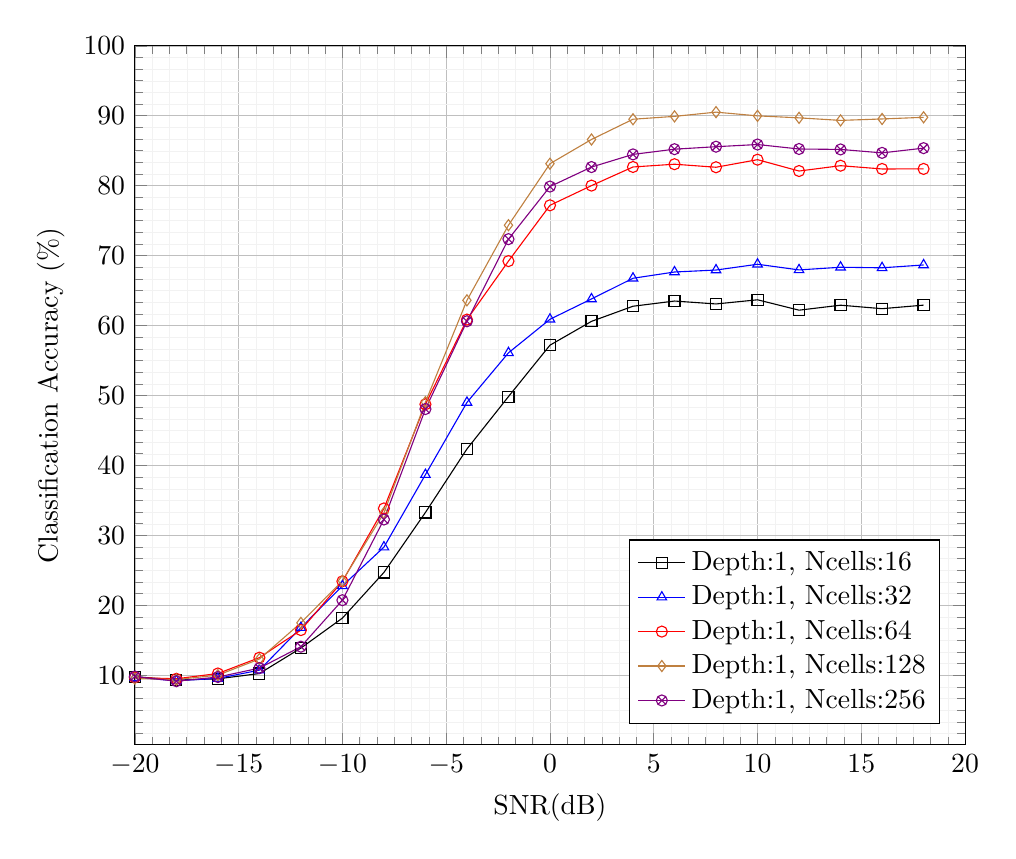
\begin{tikzpicture} \begin{axis}[legend pos=south east,
 width=\columnwidth,
 grid=both,
 ylabel=Classification Accuracy (\%),
  xlabel=SNR(dB),
 grid style={line width=.1pt, draw=gray!10},
 major grid style={line width=.2pt,draw=gray!50},
 minor tick num=5,
 xmin=-20,
 xmax=20,
 ymax=100,
 legend cell align={left},
]

\addplot[mark=square, color=black] coordinates { 
( -20 , 9.78956999085 )  ( -18 , 9.30063578565 )  ( -16 , 9.47901591896 )  ( -14 , 10.2309635511 )  ( -12 , 13.8742023701 )  ( -10 , 18.1624311356 )  ( -8 , 24.6922652949 )  ( -6 , 33.2661290323 )  ( -4 , 42.3475046211 )  ( -2 , 49.8367198839 )  ( 0 , 57.1897810219 )  ( 2 , 60.5961468557 )  ( 4 , 62.7569750367 )  ( 6 , 63.5018050542 )  ( 8 , 63.0838593327 )  ( 10 , 63.679417122 )  ( 12 , 62.1944595329 )  ( 14 , 62.9082856616 )  ( 16 , 62.407239819 )  ( 18 , 62.9162916292 )
};
\addlegendentry{Depth:1, Ncells:16}
\addplot[mark=triangle, color=blue] coordinates { 
( -20 , 9.66148215919 )  ( -18 , 9.20980926431 )  ( -16 , 9.53328509407 )  ( -14 , 10.7181522916 )  ( -12 , 16.7912488605 )  ( -10 , 22.7652390261 )  ( -8 , 28.3115928716 )  ( -6 , 38.6730205279 )  ( -4 , 49.0018484288 )  ( -2 , 56.0957910015 )  ( 0 , 60.8941605839 )  ( 2 , 63.7949836423 )  ( 4 , 66.7584434655 )  ( 6 , 67.6534296029 )  ( 8 , 67.9350766456 )  ( 10 , 68.7613843352 )  ( 12 , 67.9521998914 )  ( 14 , 68.3336408932 )  ( 16 , 68.2533936652 )  ( 18 , 68.6588658866 ) 
};
\addlegendentry{Depth:1, Ncells:32}
\addplot[mark=o, color=red] coordinates { 
( -20 , 9.66148215919 )  ( -18 , 9.48228882834 )  ( -16 , 10.2387843705 )  ( -14 , 12.5045110069 )  ( -12 , 16.4448495898 )  ( -10 , 23.4227830105 )  ( -8 , 33.8416314532 )  ( -6 , 48.7353372434 )  ( -4 , 60.8502772643 )  ( -2 , 69.2126269956 )  ( 0 , 77.1897810219 )  ( 2 , 80.0072700836 )  ( 4 , 82.6725403818 )  ( 6 , 83.0685920578 )  ( 8 , 82.6330027051 )  ( 10 , 83.7158469945 )  ( 12 , 82.093065363 )  ( 14 , 82.8566156117 )  ( 16 , 82.3891402715 )  ( 18 , 82.3942394239 ) 
};
\addlegendentry{Depth:1, Ncells:64}
\addplot[mark=diamond, color=brown] coordinates { 
( -20 , 9.51509606587 )  ( -18 , 9.37329700272 )  ( -16 , 10.003617945 )  ( -14 , 12.3060267052 )  ( -12 , 17.484047402 )  ( -10 , 23.4938688466 )  ( -8 , 33.1986037112 )  ( -6 , 49.0469208211 )  ( -4 , 63.6044362292 )  ( -2 , 74.3468795356 )  ( 0 , 83.1386861314 )  ( 2 , 86.604870956 )  ( 4 , 89.5007342144 )  ( 6 , 89.9097472924 )  ( 8 , 90.5139765555 )  ( 10 , 89.9817850638 )  ( 12 , 89.6976281007 )  ( 14 , 89.333825429 )  ( 16 , 89.5384615385 )  ( 18 , 89.7749774977 ) 
};
\addlegendentry{Depth:1, Ncells:128}
\addplot[mark=otimes, color=violet] coordinates { 
( -20 , 9.80786825252 )  ( -18 , 9.13714804723 )  ( -16 , 9.73227206946 )  ( -14 , 11.0068567304 )  ( -12 , 14.0747493163 )  ( -10 , 20.7215212369 )  ( -8 , 32.2616204299 )  ( -6 , 48.0571847507 )  ( -4 , 60.6099815157 )  ( -2 , 72.351233672 )  ( 0 , 79.8722627737 )  ( 2 , 82.6608505998 )  ( 4 , 84.4713656388 )  ( 6 , 85.2166064982 )  ( 8 , 85.572587917 )  ( 10 , 85.883424408 )  ( 12 , 85.2435270686 )  ( 14 , 85.1817678538 )  ( 16 , 84.6877828054 )  ( 18 , 85.3645364536 ) 
};
\addlegendentry{Depth:1, Ncells:256}
\end{axis}
\end{tikzpicture}
\caption{Classification accuracy of single layer amplitude-phase \ac{lstm} model for different cell size on RadioML dataset.}
\label{fig_depth_1}
\end{figure}

\subsection{Learned representations}

The inherent non-linearity and deep structures makes understanding the representations learned by \ac{lstm}s difficult. In order to obtain some good insights we use visualization techniques similar to the ones presented in \cite{vis_karpathy}. These visualizations can help to understand how \ac{lstm} cells behave for an input signal, for instance which cells gets activated at each time step and how long each gate remains open. Figures~\ref{fig_activations} and \ref{fig_gatesat} presents the gate activation and saturation of the trained two layer \ac{lstm} model for a QAM64 input signal with 18dB \ac{snr}. As explained in Section~\ref{lstm_primer} the gates of \ac{lstm} cells have sigmoid activation functions, giving an output value between 0 and 1. A gate is said to be left saturated if its activation is less than 0.1 and right saturated if the activation is greater than 0.9. The fraction of time for which the gate is in left or right saturated mode in the entire 128 samples time is plotted in Figure~\ref{fig_gatesat}. On the first layer, it can be noticed that all the three gates are confined close to the origin showing that they are not highly left or right saturated. The absence of right saturation in the first layer forget gates, confirms that the cells do not store information for long term. There are no cells in the first layer that function in purely feed-forward fashion, since their forget gates would show up as consistently left-saturated. The output gate plots in the first layer also show that there are no cells that are revealed or blocked to the hidden state. This is also visible in the activation plots of the first layer in Figure~\ref{fig_activations}. The activations are short when compared to the second layer and it can be noticed in Figure~\ref{fig_activations} that many cell activations follow the input amplitude and phase changes in the input waveform. The second layer stores much long term dependencies from the fine grained representations generated from the first layer. 


% \begin{figure*}
% \begin{minipage}[c][20cm][t]{.3\textwidth}
%   \vspace*{\fill}
%   \centering
%   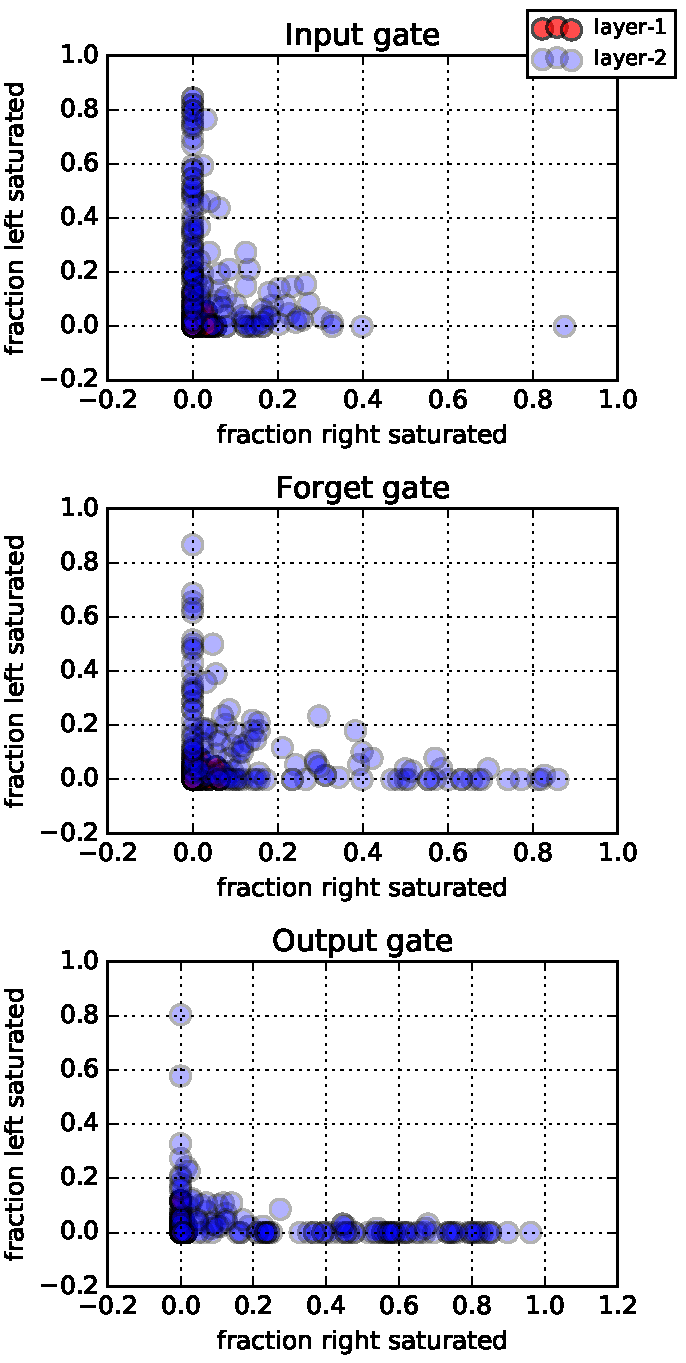
\includegraphics[width=\columnwidth,height=10cm]{figures/gate_sat_vert.pdf}
%   \caption{test figure one}
%   \label{fig:test1}
% \end{minipage}%
% \begin{minipage}[c][20cm][t]{.7\textwidth}
%   \vspace*{\fill}
%   \centering
%   \includegraphics[width=\columnwidth,height=10cm]{figures/layer_1.pdf}
%   \caption{test figure two}
%   \label{fig:test2}\par\vfill
%   \includegraphics[width=\columnwidth,height=10cm]{figures/layer_2.pdf}
%   \caption{test figure three}
%   \label{fig:test3}
% \end{minipage}
% \end{figure*}



% \begin{figure}[!t]
% \centering
% \squeezeup
% 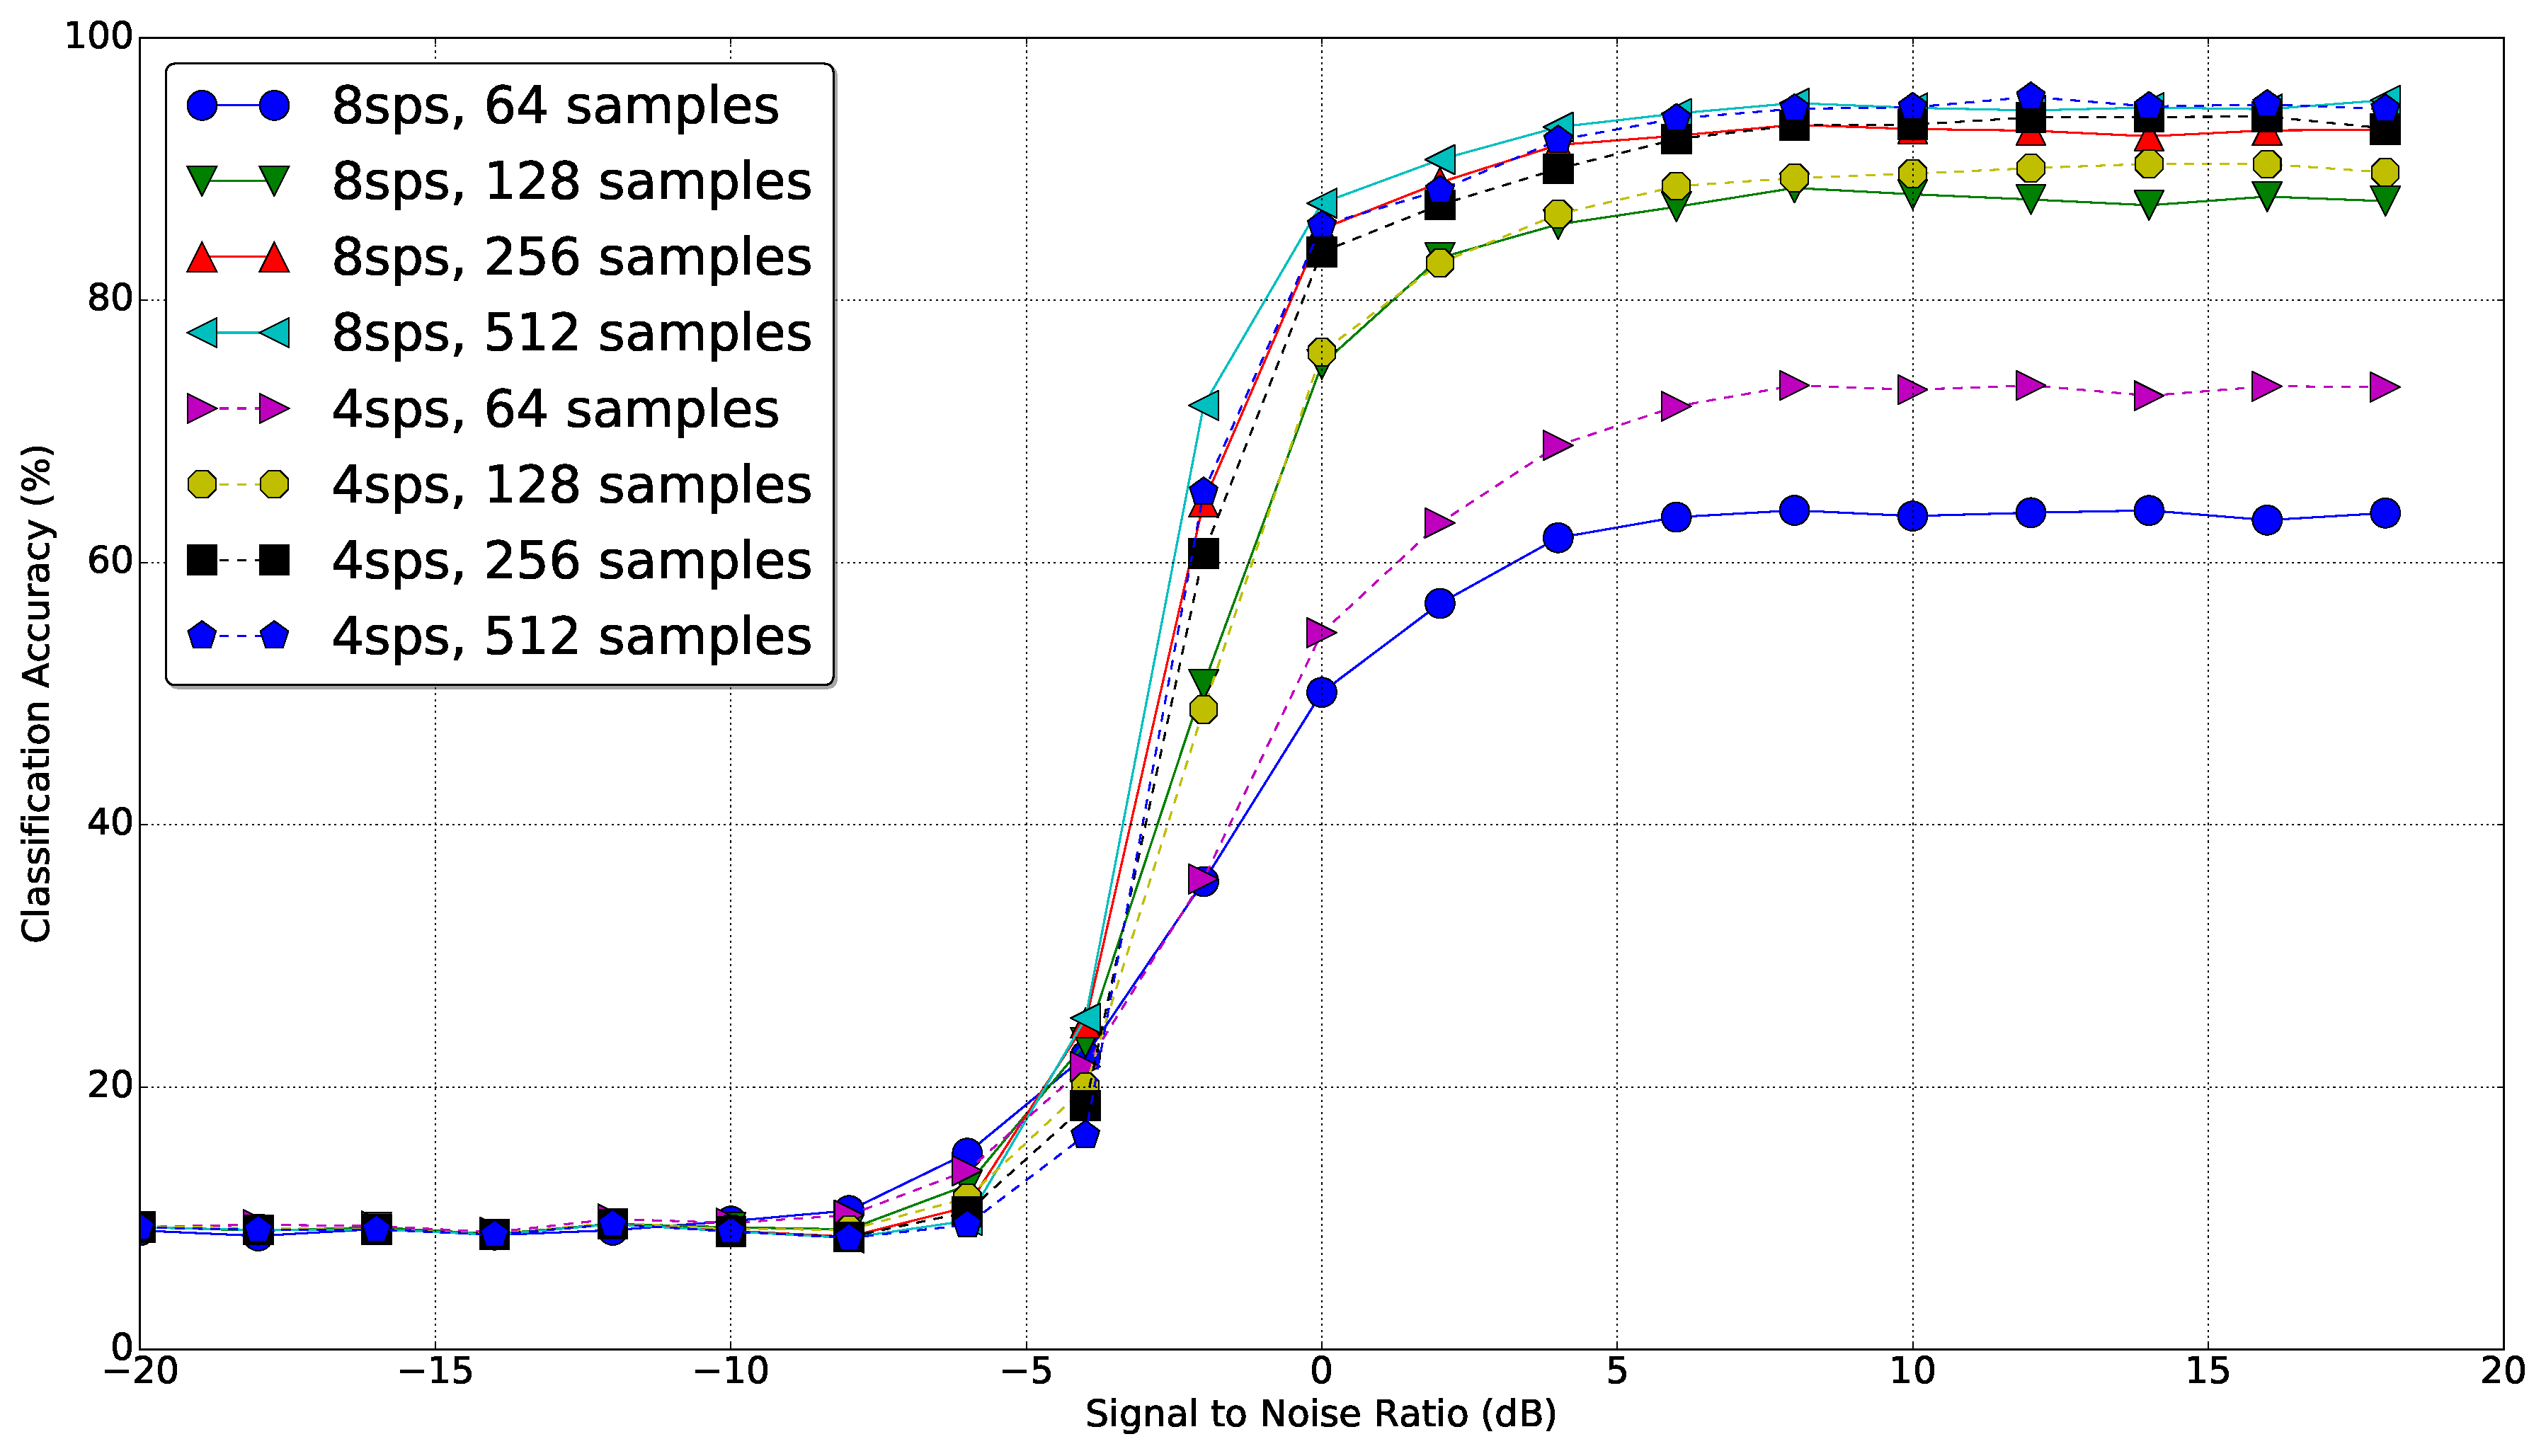
\includegraphics[width=\columnwidth]{sections/lstm_accuracy.pdf}
% \caption{Classification accuracy for a model trained only on high SNR signals.}
% \label{fig_high_snr}
% \end{figure}

% \begin{figure}[!t]
% \centering
% \squeezeup
% %\resizebox{\columnwidth}{!}{\input{lstm_accuracy_lowsnr.pgf}}
% 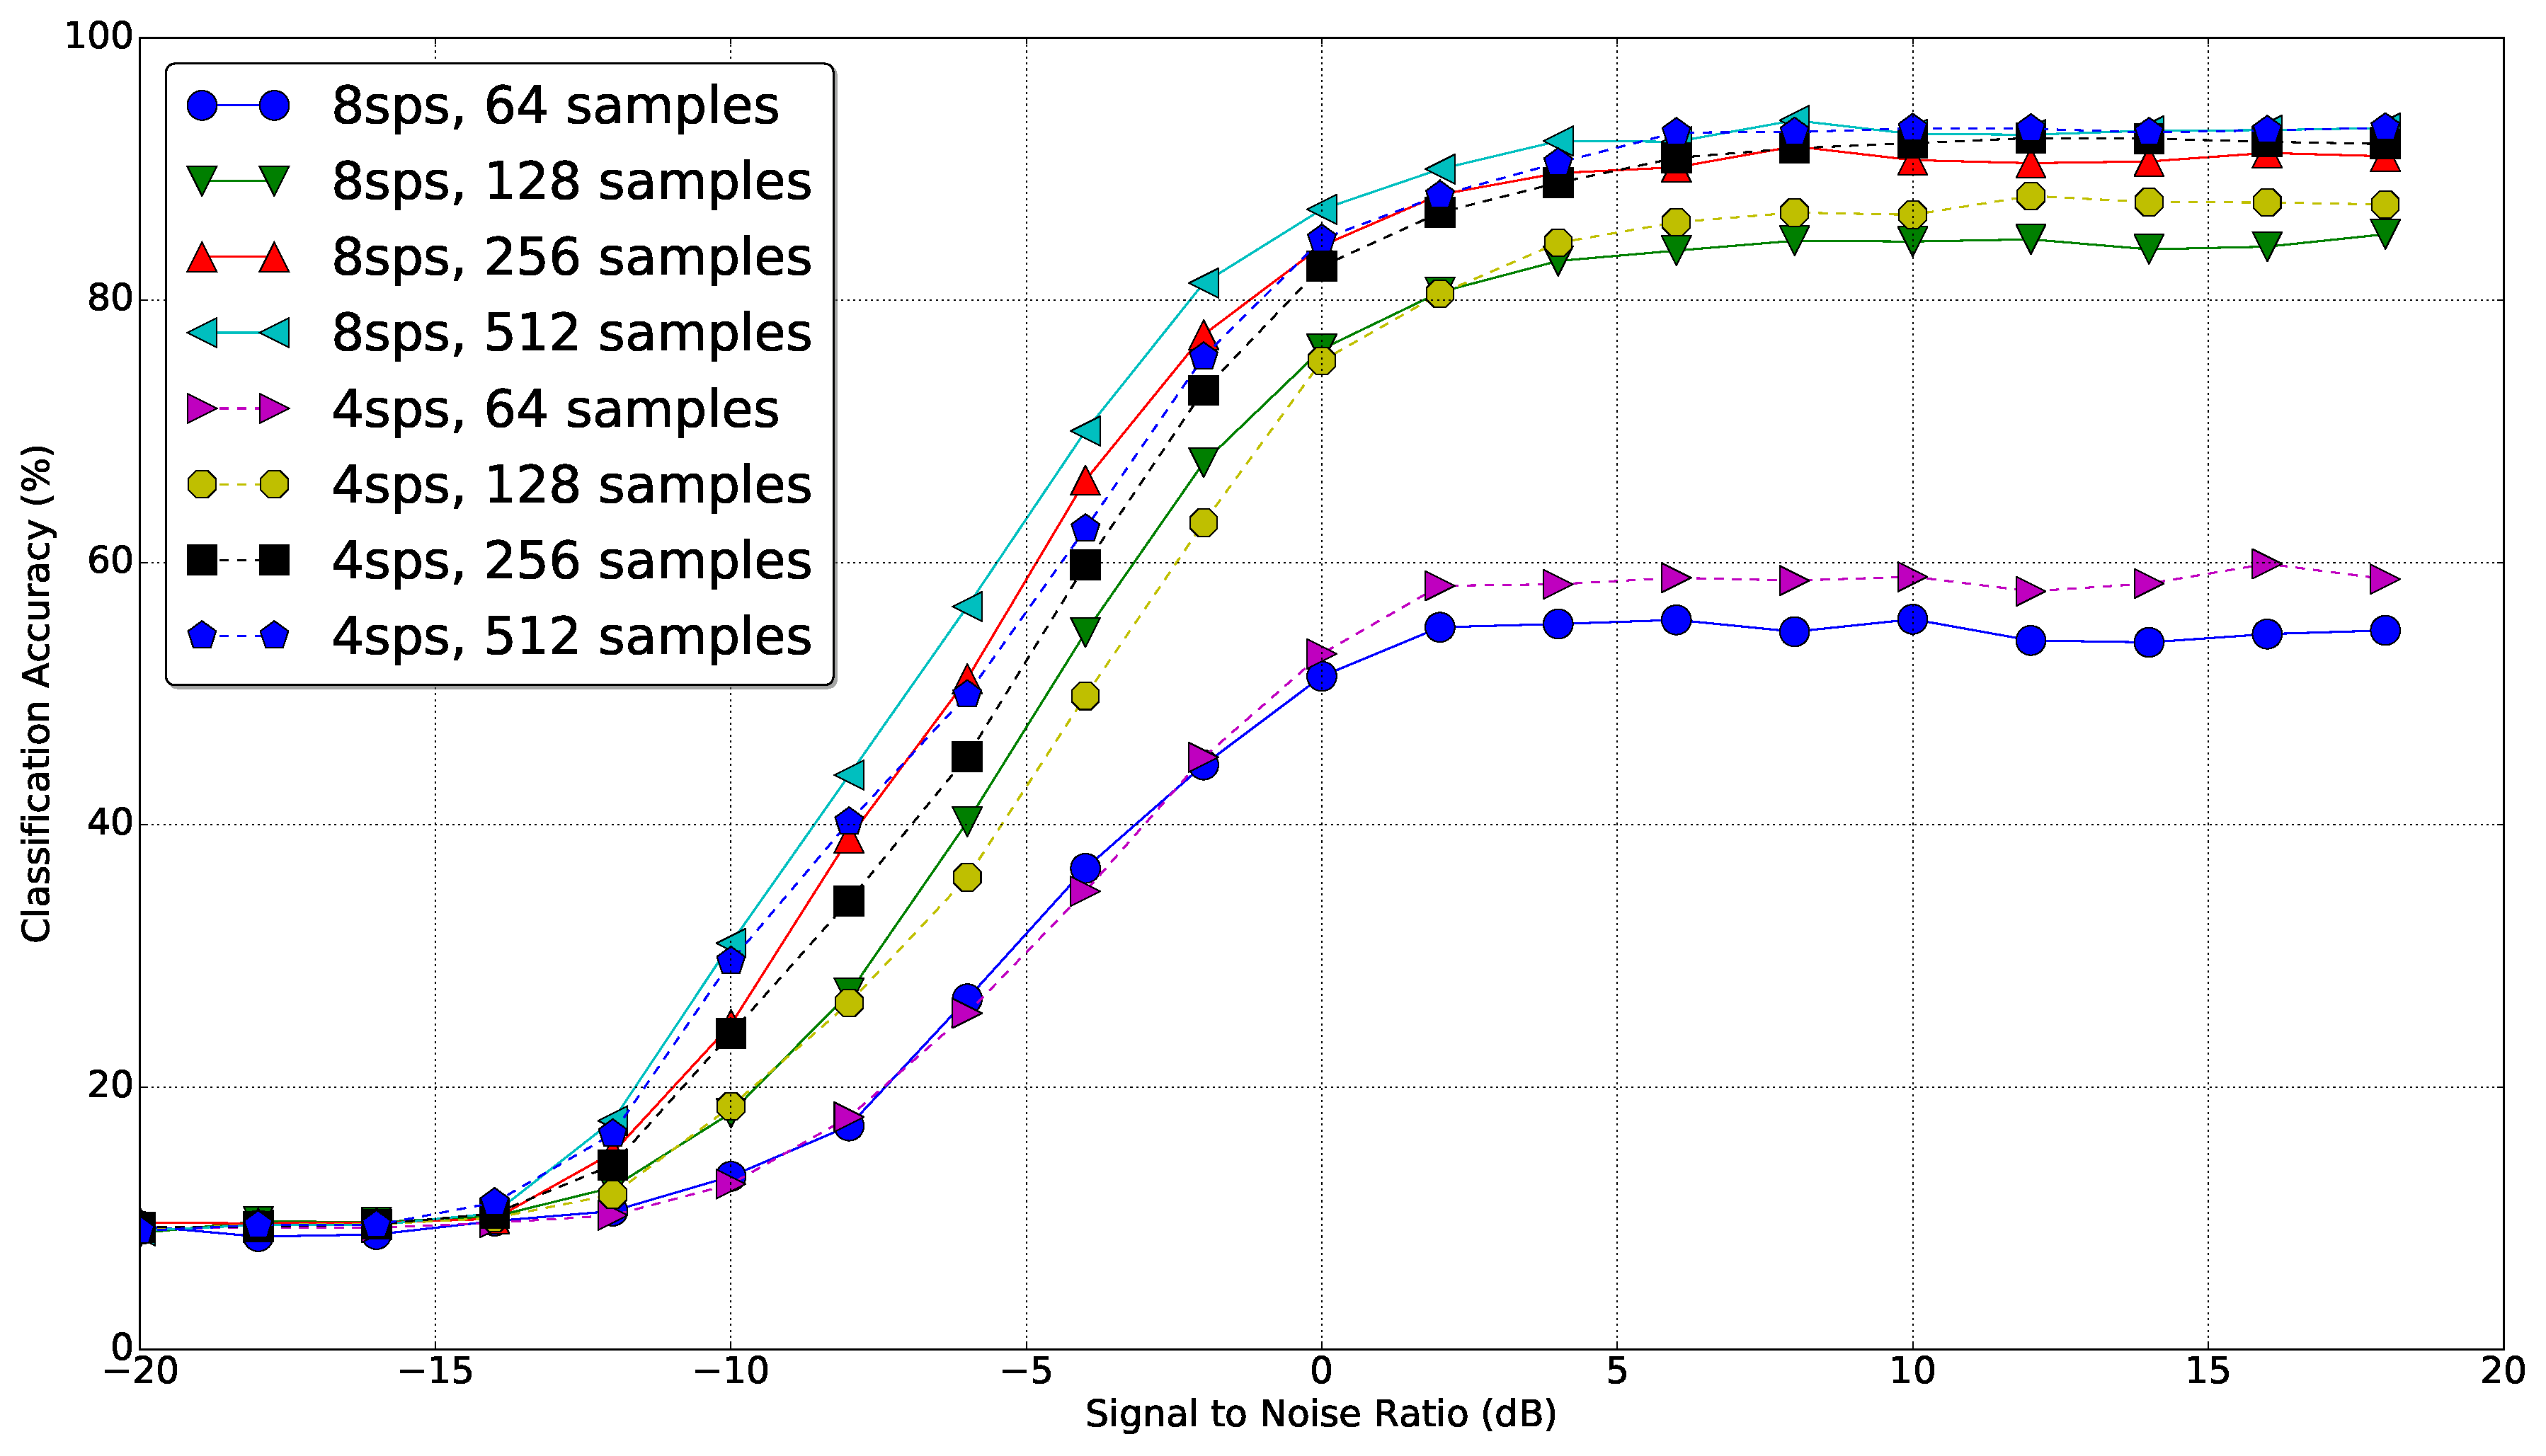
\includegraphics[width=\columnwidth]{sections/lstm_accuracy_lowsnr.pdf}
% \caption{Classification accuracy for a model trained on signals of all SNRs.}
% \label{fig_low_snr}
% \end{figure}



% \subsection{Performance comparison with CNN, and Cyclostationary models on RadioML dataset}
% \begin{itemize}
% \item Cyclostationary moments should be generated and we need to make sure that the selected moments/cumulants make sense. Please see Chad's analysis in his \href{https://cyclostationary.blog/2017/01/31/machine-learning-and-modulation-recognition-comments-on-convolutional-radio-modulation-recognition-networks-by-t-oshea-j-corgan-and-t-clancy/}{blog}.
% \item A little bit time consuming
% \end{itemize}

\subsection{Effect of cell size and layer depth}
\label{sec_hyperparams}


\begin{figure}[htb]
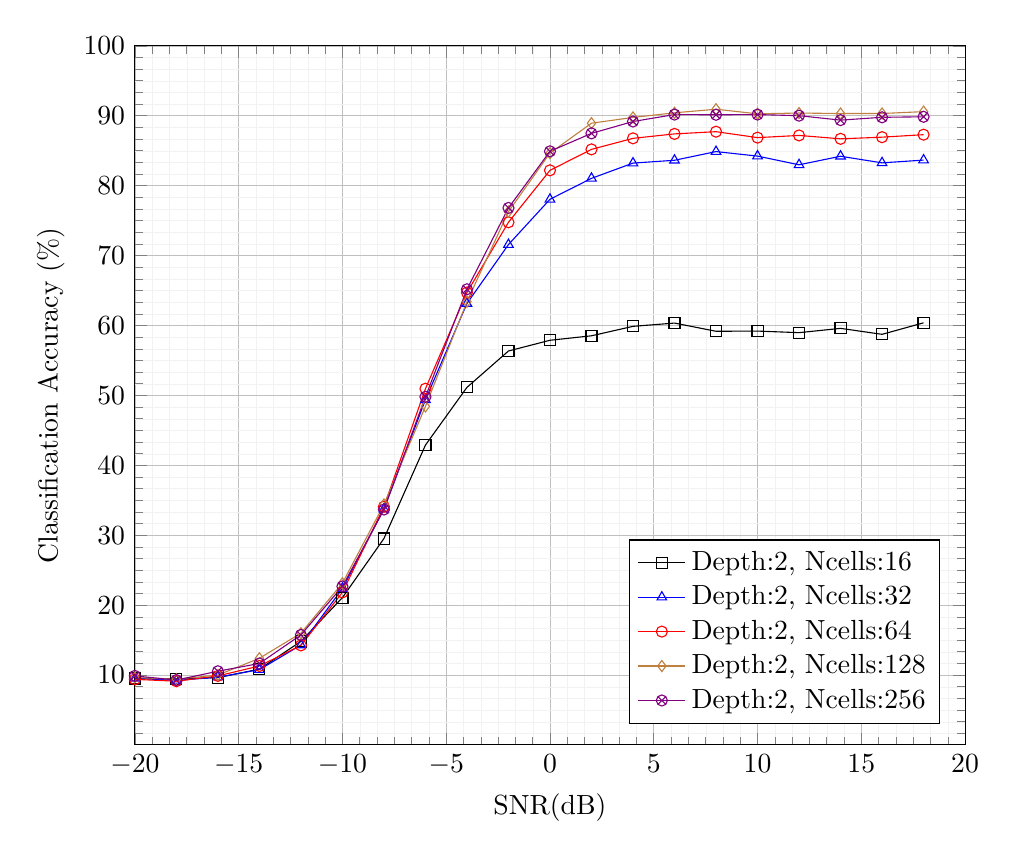
\begin{tikzpicture} \begin{axis}[legend pos=south east,
 width=\columnwidth,
 grid=both,
 ylabel=Classification Accuracy (\%),
  xlabel=SNR(dB),
 grid style={line width=.1pt, draw=gray!10},
 major grid style={line width=.2pt,draw=gray!50},
 minor tick num=5,
 xmin=-20,
 xmax=20,
 ymax=100,
 legend cell align={left},
]

\addplot[mark=square, color=black] coordinates { 
( -20 , 9.51509606587 )  ( -18 , 9.46412352407 )  ( -16 , 9.62373371925 )  ( -14 , 10.8444604836 )  ( -12 , 14.8040109389 )  ( -10 , 21.0769504176 )  ( -8 , 29.5241594709 )  ( -6 , 42.8885630499 )  ( -4 , 51.146025878 )  ( -2 , 56.3497822932 )  ( 0 , 57.8832116788 )  ( 2 , 58.524173028 )  ( 4 , 59.8751835536 )  ( 6 , 60.3429602888 )  ( 8 , 59.1704238052 )  ( 10 , 59.1985428051 )  ( 12 , 58.9715734202 )  ( 14 , 59.5866396014 )  ( 16 , 58.7330316742 )  ( 18 , 60.3780378038 ) 
};
\addlegendentry{Depth:2, Ncells:16}
\addplot[mark=triangle, color=blue] coordinates { 
( -20 , 9.53339432754 )  ( -18 , 9.22797456857 )  ( -16 , 9.69609261939 )  ( -14 , 10.7722843739 )  ( -12 , 14.2935278031 )  ( -10 , 22.3742669273 )  ( -8 , 33.731398126 )  ( -6 , 49.3768328446 )  ( -4 , 63.1423290203 )  ( -2 , 71.5711175617 )  ( 0 , 78.0474452555 )  ( 2 , 81.0432569975 )  ( 4 , 83.2232011747 )  ( 6 , 83.6281588448 )  ( 8 , 84.869251578 )  ( 10 , 84.2258652095 )  ( 12 , 82.9802643491 )  ( 14 , 84.203727625 )  ( 16 , 83.257918552 )  ( 18 , 83.6543654365 ) 
};
\addlegendentry{Depth:2, Ncells:32}
\addplot[mark=o, color=red] coordinates { 
( -20 , 9.38700823422 )  ( -18 , 9.11898274296 )  ( -16 , 9.87698986975 )  ( -14 , 11.2955611693 )  ( -12 , 14.2388331814 )  ( -10 , 21.8233516972 )  ( -8 , 34.0804703289 )  ( -6 , 50.9530791789 )  ( -4 , 64.7134935305 )  ( -2 , 74.7641509434 )  ( 0 , 82.1897810219 )  ( 2 , 85.1872046529 )  ( 4 , 86.7657856094 )  ( 6 , 87.4007220217 )  ( 8 , 87.7186654644 )  ( 10 , 86.8670309654 )  ( 12 , 87.1808799565 )  ( 14 , 86.6949621701 )  ( 16 , 86.9321266968 )  ( 18 , 87.2907290729 ) 
};
\addlegendentry{Depth:2, Ncells:64}
\addplot[mark=diamond, color=brown] coordinates {
( -20 , 9.64318389753 )  ( -18 , 9.40962761126 )  ( -16 , 10.003617945 )  ( -14 , 12.3962468423 )  ( -12 , 15.9890610757 )  ( -10 , 23.1384396659 )  ( -8 , 34.3927980893 )  ( -6 , 48.4237536657 )  ( -4 , 63.4011090573 )  ( -2 , 76.2880986938 )  ( 0 , 84.6532846715 )  ( 2 , 88.9312977099 )  ( 4 , 89.7577092511 )  ( 6 , 90.4151624549 )  ( 8 , 90.9287646528 )  ( 10 , 90.2732240437 )  ( 12 , 90.3856599674 )  ( 14 , 90.3118656579 )  ( 16 , 90.3167420814 )  ( 18 , 90.5850585059 ) 
};
\addlegendentry{Depth:2, Ncells:128}
\addplot[mark=otimes, color=violet] coordinates { 
( -20 , 9.88106129918 )  ( -18 , 9.28247048138 )  ( -16 , 10.5463096961 )  ( -14 , 11.6564417178 )  ( -12 , 15.7338195077 )  ( -10 , 22.6763817309 )  ( -8 , 33.6762814624 )  ( -6 , 49.7983870968 )  ( -4 , 65.1756007394 )  ( -2 , 76.8142235123 )  ( 0 , 84.9087591241 )  ( 2 , 87.4772809887 )  ( 4 , 89.1703377386 )  ( 6 , 90.1624548736 )  ( 8 , 90.1352569883 )  ( 10 , 90.1639344262 )  ( 12 , 90.0054318305 )  ( 14 , 89.3707326075 )  ( 16 , 89.7737556561 )  ( 18 , 89.8469846985 ) 
};
\addlegendentry{Depth:2, Ncells:256}
\end{axis}
\end{tikzpicture}
\caption{Classification accuracy of two layer amplitude-phase \ac{lstm} model for different cell sizes on RadioML dataset.}
\label{fig_depth_2}
\end{figure}



\begin{figure}[htb]
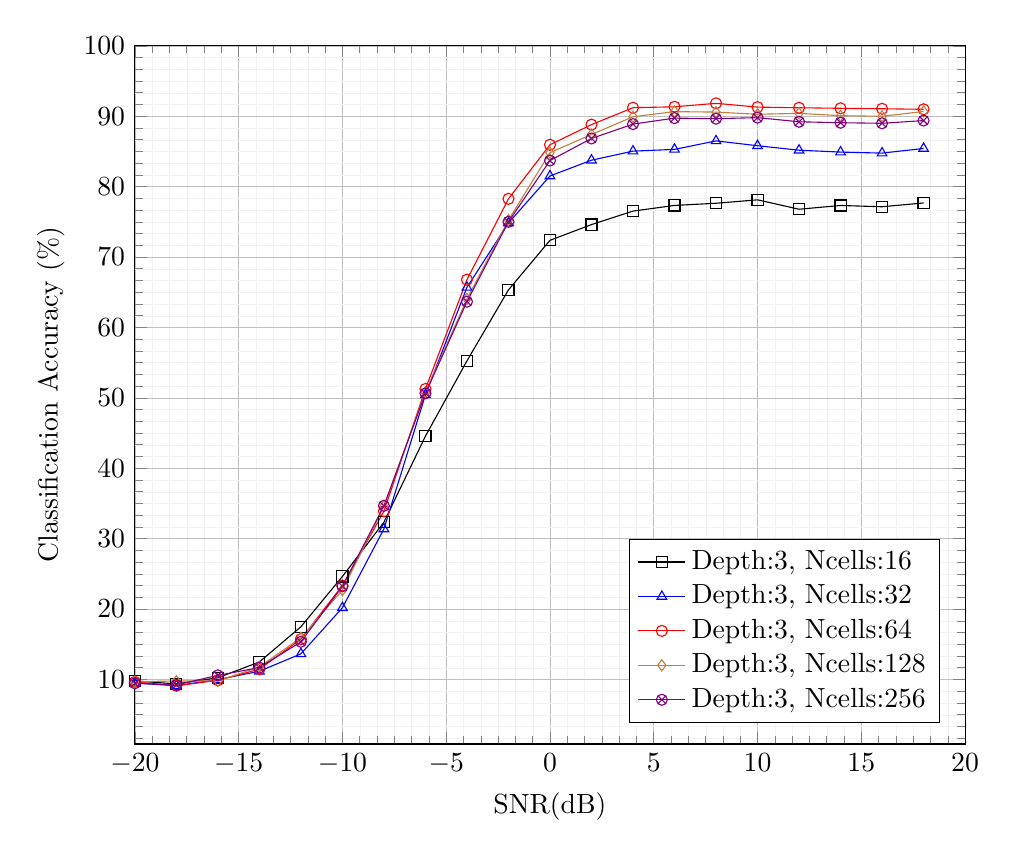
\begin{tikzpicture} \begin{axis}[legend pos=south east,
 width=\columnwidth,
 grid=both,
 ylabel=Classification Accuracy (\%),
  xlabel=SNR(dB),
 grid style={line width=.1pt, draw=gray!10},
 major grid style={line width=.2pt,draw=gray!50},
 minor tick num=5,
 xmin=-20,
 xmax=20,
 legend cell align={left},
]

\addplot[mark=square, color=black] coordinates { 
( -20 , 9.78956999085 )  ( -18 , 9.37329700272 )  ( -16 , 10.2387843705 )  ( -14 , 12.4864669794 )  ( -12 , 17.484047402 )  ( -10 , 24.631242225 )  ( -8 , 32.3351093147 )  ( -6 , 44.5564516129 )  ( -4 , 55.2495378928 )  ( -2 , 65.3301886792 )  ( 0 , 72.3722627737 )  ( 2 , 74.6092330062 )  ( 4 , 76.5234948605 )  ( 6 , 77.3285198556 )  ( 8 , 77.6375112714 )  ( 10 , 78.1238615665 )  ( 12 , 76.7879775484 )  ( 14 , 77.3205388448 )  ( 16 , 77.1402714932 )  ( 18 , 77.6777677768 ) 
};
\addlegendentry{Depth:3, Ncells:16}
\addplot[mark=triangle, color=blue] coordinates { 
( -20 , 9.47849954254 )  ( -18 , 9.11898274296 )  ( -16 , 9.98552821997 )  ( -14 , 11.1692529773 )  ( -12 , 13.6371923428 )  ( -10 , 20.1883774658 )  ( -8 , 31.3797538122 )  ( -6 , 50.4215542522 )  ( -4 , 65.6931608133 )  ( -2 , 74.8367198839 )  ( 0 , 81.5145985401 )  ( 2 , 83.7513631407 )  ( 4 , 85.0403817915 )  ( 6 , 85.2888086643 )  ( 8 , 86.4923354373 )  ( 10 , 85.810564663 )  ( 12 , 85.1711026616 )  ( 14 , 84.9049640155 )  ( 16 , 84.7601809955 )  ( 18 , 85.4185418542 ) 
};
\addlegendentry{Depth:3, Ncells:32}
\addplot[mark=o, color=red] coordinates { 
( -20 , 9.66148215919 )  ( -18 , 9.10081743869 )  ( -16 , 9.87698986975 )  ( -14 , 11.4579574161 )  ( -12 , 15.7338195077 )  ( -10 , 23.3339257153 )  ( -8 , 33.8967481168 )  ( -6 , 51.2646627566 )  ( -4 , 66.7837338262 )  ( -2 , 78.2656023222 )  ( 0 , 85.9489051095 )  ( 2 , 88.8040712468 )  ( 4 , 91.2077826725 )  ( 6 , 91.3357400722 )  ( 8 , 91.830477908 )  ( 10 , 91.2932604736 )  ( 12 , 91.2004345464 )  ( 14 , 91.1238235837 )  ( 16 , 91.0588235294 )  ( 18 , 90.9810981098 ) 
};
\addlegendentry{Depth:3, Ncells:64}
\addplot[mark=diamond, color=brown] coordinates { 
( -20 , 9.69807868253 )  ( -18 , 9.77293369664 )  ( -16 , 9.80463096961 )  ( -14 , 11.7827499098 )  ( -12 , 15.934366454 )  ( -10 , 22.69415319 )  ( -8 , 34.5948925225 )  ( -6 , 50.7881231672 )  ( -4 , 64.0480591497 )  ( -2 , 75.2539912917 )  ( 0 , 84.8175182482 )  ( 2 , 87.4045801527 )  ( 4 , 89.922907489 )  ( 6 , 90.6498194946 )  ( 8 , 90.5861136159 )  ( 10 , 90.2732240437 )  ( 12 , 90.4037660692 )  ( 14 , 90.071968998 )  ( 16 , 89.9909502262 )  ( 18 , 90.6750675068 )
};
\addlegendentry{Depth:3, Ncells:128}
\addplot[mark=otimes, color=violet] coordinates { 
( -20 , 9.46020128088 )  ( -18 , 9.22797456857 )  ( -16 , 10.5824891462 )  ( -14 , 11.6925297726 )  ( -12 , 15.3509571559 )  ( -10 , 23.2272969611 )  ( -8 , 34.6683814073 )  ( -6 , 50.6414956012 )  ( -4 , 63.6598890943 )  ( -2 , 75.0 )  ( 0 , 83.704379562 )  ( 2 , 86.8411486732 )  ( 4 , 88.8766519824 )  ( 6 , 89.7292418773 )  ( 8 , 89.6483318305 )  ( 10 , 89.7996357013 )  ( 12 , 89.2087633533 )  ( 14 , 89.0754751799 )  ( 16 , 88.9954751131 )  ( 18 , 89.3789378938 )
};
\addlegendentry{Depth:3, Ncells:256}
\end{axis}
\end{tikzpicture}
\caption{Classification accuracy of three layer amplitude-phase \ac{lstm} model for different cell sizes on RadioML dataset.}
\label{fig_depth_3}
\end{figure}

A comprehensive study is also performed to understand the effect of the number cells and layer depth on the model performance. The number of \ac{lstm} cells and layer depth are varied from 16 to 256 and  1 to 3 respectively. The models are trained on RadioML dataset on all \ac{snr}s. The accuracy levels for various layer depths are presented in Figures~\ref{fig_depth_1}, \ref{fig_depth_2} and \ref{fig_depth_3}. An initial analysis clearly shows that the model accuracy increases with increasing layer depth for mostly all cell sizes. It can be also noted that as the depth of the model increases, increasing the number of cells doesn't give much performance improvements. For instance, at depths 2 and 3 increasing the cell numbers from 128 to 256 doesn't provide any performance improvements.




% \subsection{Classification accuracy on real-life data}
% Add over the air results

